\section{Next steps in the investigation of the PMNS matrix}
\label{sec:future}

Following the precise measurement of \thint we know that all the three mixing angles of the PMNS matrix are different from zero, opening the possibility of having CP violation in the leptonic sector. The discovery of this new source of CP violation, corresponding to the observation of a sin\dcp different from zero, could be an important step in our understanding of the baryon asymmetry in the Universe and will be the main goal of the long baseline accelerator experiments in the coming years. As of today, data are compatible with most of the values of \dcp, although indications from T2K show a preference for $\dcp\sim-\pi/2$ excluding at more than 3$\sigma$ values of \dcp close to \pipi/2 and excluding CP conservation at 90\% CL. 

In addition to the measurement of \dcp, other questions have still to be addressed before having a complete picture of the neutrino oscillations: in particular, as explained in~\ref{} the mass ordering between the eigenstate $\nu_3$ and the other two is still unknown. The ordering can be normal ($m_3 > m_2 > m_1$) or inverted ($m_2 > m_1 > m_3$) and, knowing the ordering, will have important consequences on the nature of the neutrinos. For example, the sensitivity required for the observation of neutrinoless double beta decay, that would prove that neutrinos are Majorana particles, is much larger if the ordering is normal. The question of ordering has also an impact on cosmology, where measurements are getting closer to be sensitive to the sum of the masses of the three neutrinos, and for model builders. In fact most Grand Unified Model predict a normal ordering.

The mass ordering has also a direct impact on \dcp. As we have shown in Sect.~\ref{}, degeneracies exist in the \nue appearance probability in long-baseline experiments between \dcp and the mass ordering. If this latter parameter will be measured, the degeneracy will be solved and the measurement of \dcp will be easier.

Another important question to be addressed is the precise measurement of \thatm. Currently the value of this mixing angle is compatible with $\pi/4$ that give the so-called maximal disappearance, since the \num disappearance probability is proportional to \sttt. This is known as the octant degeneracy since, values of \thatm of $\pi/4+X$ or $\pi/4-X$ give the same disappearance probability. Nevertheless, precise measurements of different oscillation channels, allow to disentangle among the two solutions and determine in which octant \thatm stands if $X$ is large enough. A value of \thatm exactly equal to $\pi/4$ is particularly interesting because it might indicate the existence of an underlying symmetry.

This section is organized as follow. We will first review the sensitivity of the running long-baseline experiments (T2K and \nova) that might give some indications of CP violation, mass ordering and the \thatm octant in the coming years. We will then review the non-accelerator based experiments (JUNO, PINGU, ORCA and INO) that have some sensitivity to the mass ordering and finally we will describe the future long-baseline accelerator experiments (HyperKamiokande and DUNE) whose main goal is to observe the CP violation in the leptonic sector, performing a precise measurement of \dcp. 


\subsection{Goals of the running experiments: T2K and \nova}
\label{sec:futuret2knova}

In the next $\sim10$ years there will be no new long-baseline experiment; however the running experiments, T2K and \nova, will greatly increase their statistics, collecting $\sim10$ times more data with respect to what has been collected and analysed so far. 

T2K has presented results based on a total of $1.5 \times10^{21}$ protons-on-target (\pot) while the total expected statistics for which the experiment had been approved is $7.8\times10^{21}$ \pot. Such a statistics, that will be collected by 2020, corresponded to the need to maximize the sensitivity to small values of \thint that at the time of the T2K proposal was unknown. Today we know very precisely the value of \thint and its large value implies that the T2K sensitivity to \dcp is statistically limited at $7.8\times10^{21}$ \pot and will benefit of a larger exposure. 

For this reason the collaboration has recently submitted a proposal for the so-called T2K phase II~\cite{Abe:2016tez}. During this phase, that will take place from 2020 to 2026, a total of  $20\times10^{21}$~\pot will be collected, and this will allow to exclude CP conservation at more than 3 sigma if the true value of \dcp is close to the values that maximally violate CP.

The other running experiment, \nova, has so-far presented results based on $\sim6\times10^20$ \pot while the experiment is expected to collect $36\times10^{20}$ \pot by 2020. 

The two experiments are highly complementary thanks to the different baseline. The longer \nova baseline allows this experiment to have a better sensitivity to the matter effects and therefore to the mass ordering while for T2K, the matter effects are small and the experiment is mostly sensitive to \dcp. In the case of \nova, in fact, the two mass ordering solutions lead to a difference in the \nue appearance probability of $\pm19\%$ while the two maximal cases of CP violation, $\dcp=-\pi/2$ and $\pi/2$ lead to a difference in the \nue appearance probability of $\pm22\%$. In the case of T2K, instead, the mass ordering has an effect of $\pm10\%$ on the appearance probability while the two maximal CP violation cases lead to a difference of $\pm29\%$. 

With $20\times10^{21}$ \pot, equally split in neutrino and anti-neutrino mode, and some realistic improvements in the analyses, T2K will observe $\sim500$ ($\sim100$) e-like candidates in neutrino (anti-neutrino) mode as well as $\sim2700$ ($\sim1300$) \mmu-like candidates. The sensitivity to \dcp with such statistics is shown in Fig.~\ref{fig:t2k2sensi}, in the two cases of known or unknown mass ordering. The knowledge of the mass ordering would greatly impact the sensitivity to positive values of \dcp (assuming normal ordering). This is due to the degeneracy between the normal ordering and positive values of \dcp since the first tends to increase the number of \nue appearance candidates while the latter tends to reduce it. For negative values of \dcp instead, there is no degeneracy since normal ordering and positive \dcp would both tend to increase the \nue appearance probability. In this sensitivity study an improvement of the systematic uncertainties in the T2K analyses is also assumed. To reach such improvements an upgrade of the Near Detector complex is under discussion within the collaboration. Assuming the mass ordering to be determined by another experiment and that the reduction of the systematic uncertainties is obtained, the fractional region for which \(\sin\delta_{CP}=0\) can be excluded at the 99\% (3\(\sigma\)) C.L.\ is 49\% (36\%) of possible true values of \dcp. Without improvements on the systematic uncertainties, the corresponding fractions are 42$\%$ (21$\%$). These results mildly depend on the value of \stt, the sensitivity being slightly better for the lower octant solution.

\begin{figure} [htbp!]
\begin{center}
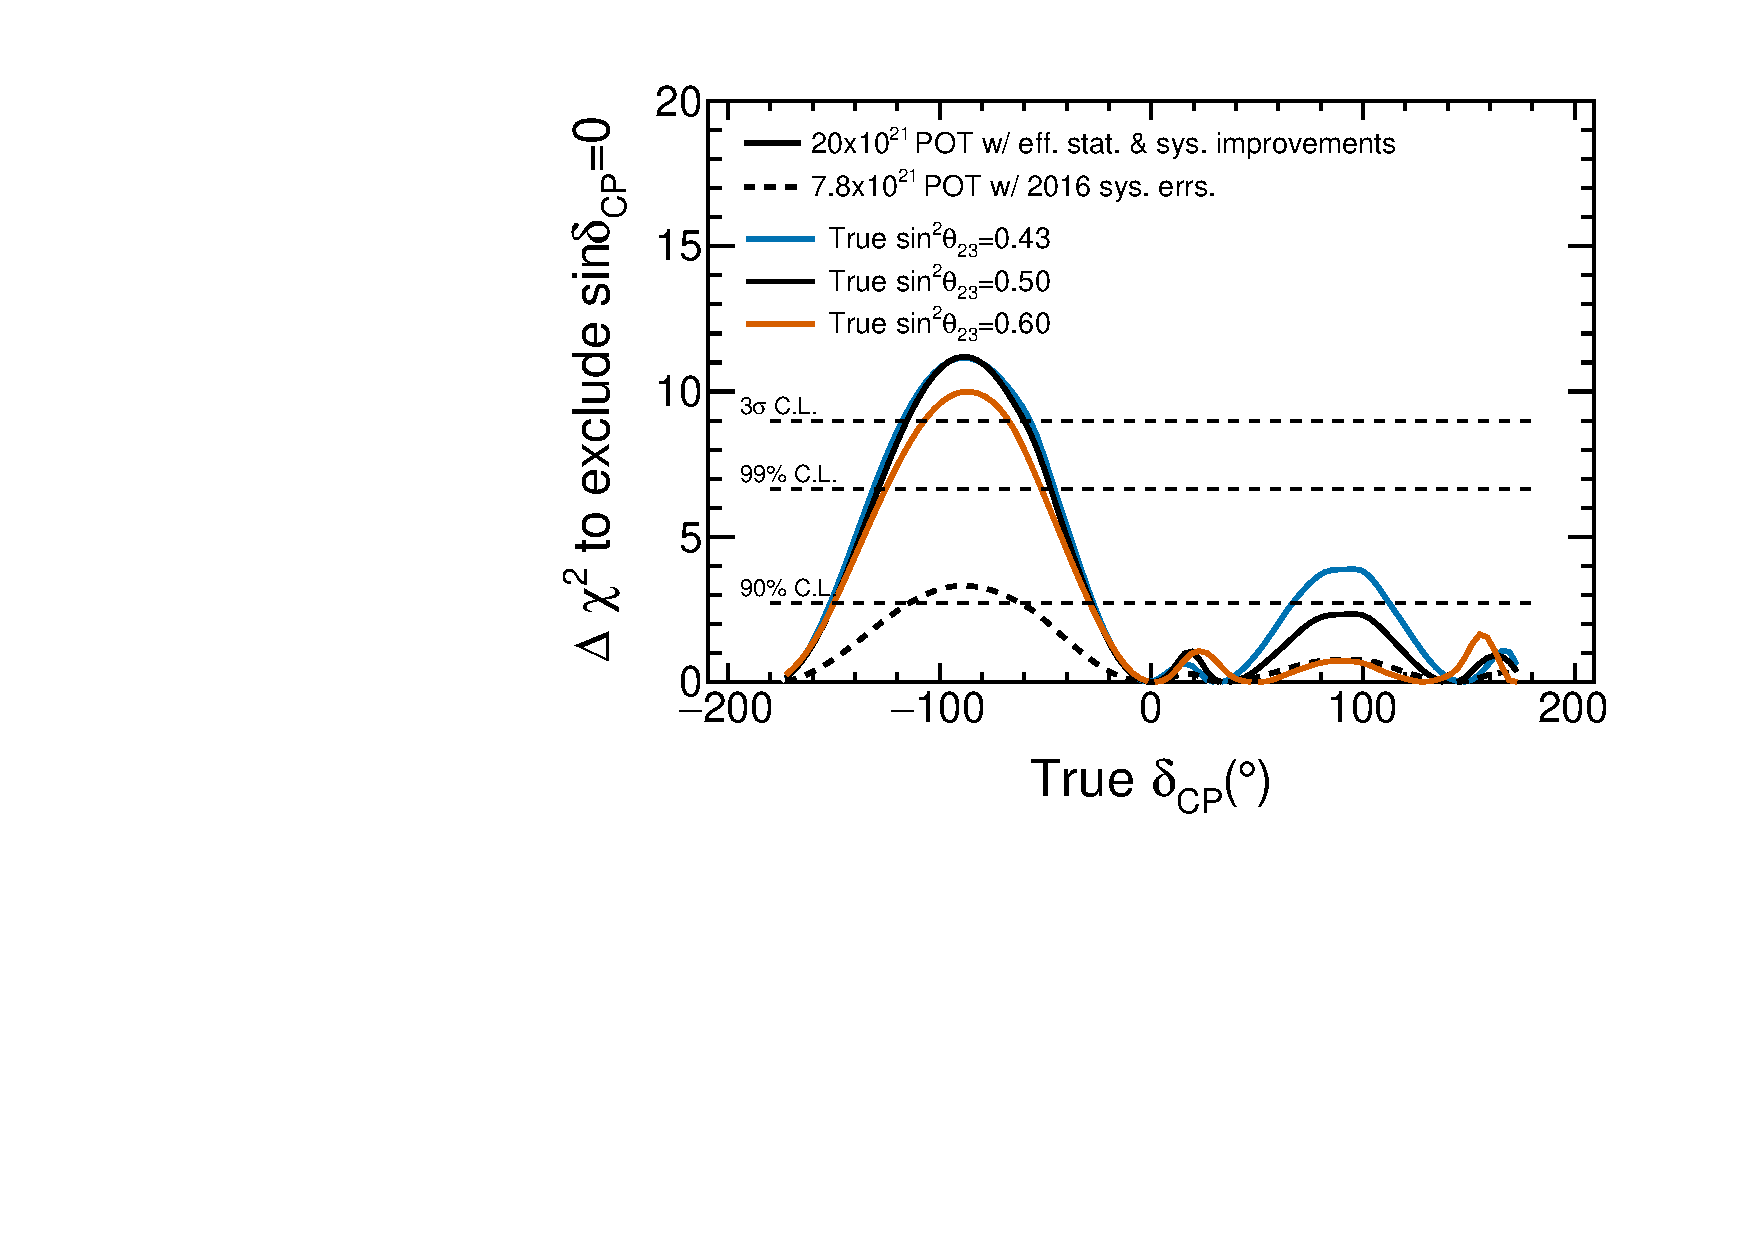
\includegraphics[width=8cm]{figures/t2kpre_dcp_point1_100k4check_100ksensi_wreactorthrow_optv2s13off_truedcp_unknownMH_fakesyst_lohidcpExclusive.pdf}
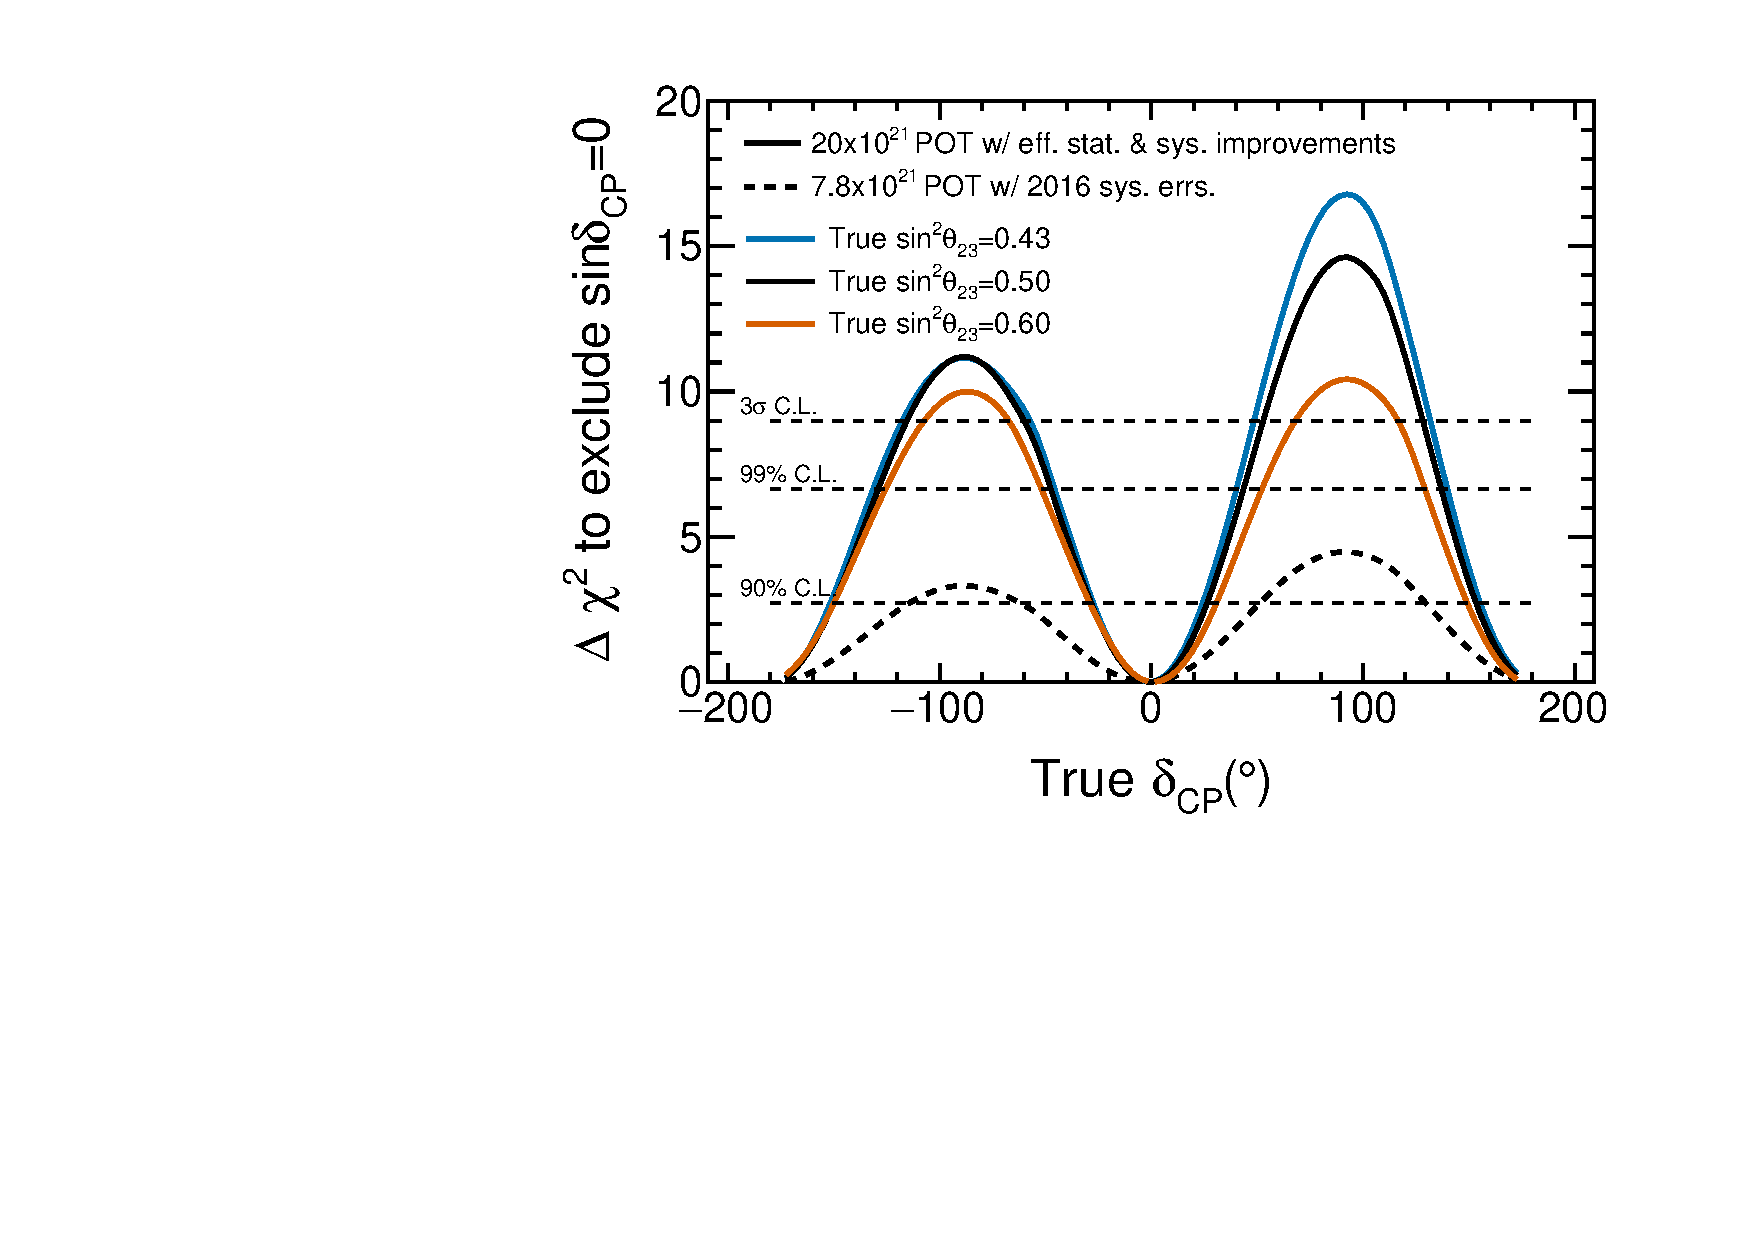
\includegraphics[width=8cm]{figures/t2kpre_dcp_point1_100k4check_100ksensi_wreactorthrow_optv2s13off_truedcp_fakesyst_lohidcpExclusive.pdf}
\caption{\label{fig:t2k2sensi} Sensitivity to CP violation as a function of true
\dcp with three values of \stt (0.43, 0.50, 0.60) and normal hierarchy for the full T2K-II exposure of \twopott and a reduction of the systematic error to 2/3 of the 2016 T2K uncertainties. On the left plot the mass ordering is considered unknown while on the right plot it is considered known.~\cite{Abe:2016tez}.}
\end{center}
\end{figure}

With such statistics T2K will also be able to perform leading measurement of the \stt mixing angle as is shown in Fig.~\ref{fig:t2k2th23}.

\begin{figure} [htbp!]
\begin{center}
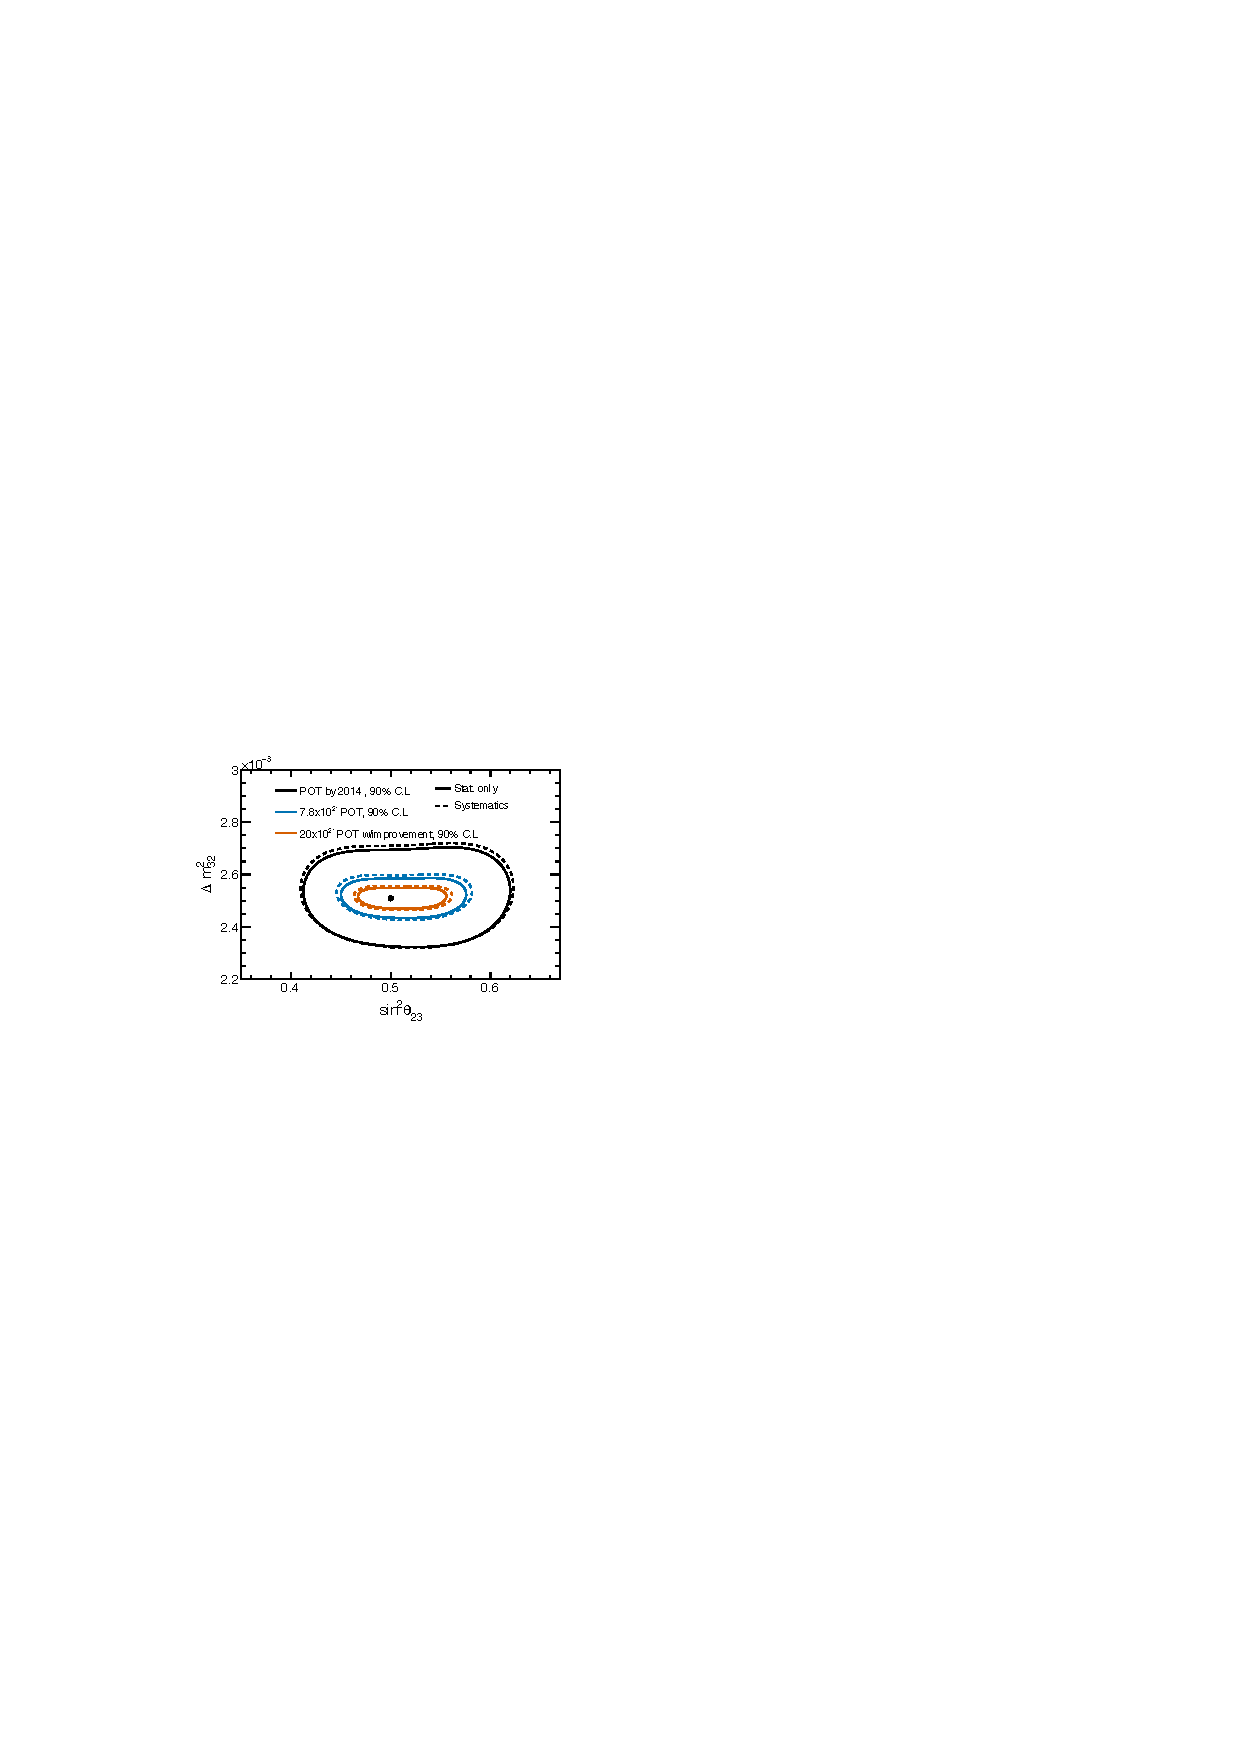
\includegraphics[width=8cm]{figures/t2kpre_t23dm32_point1_wreactorthrow.pdf}
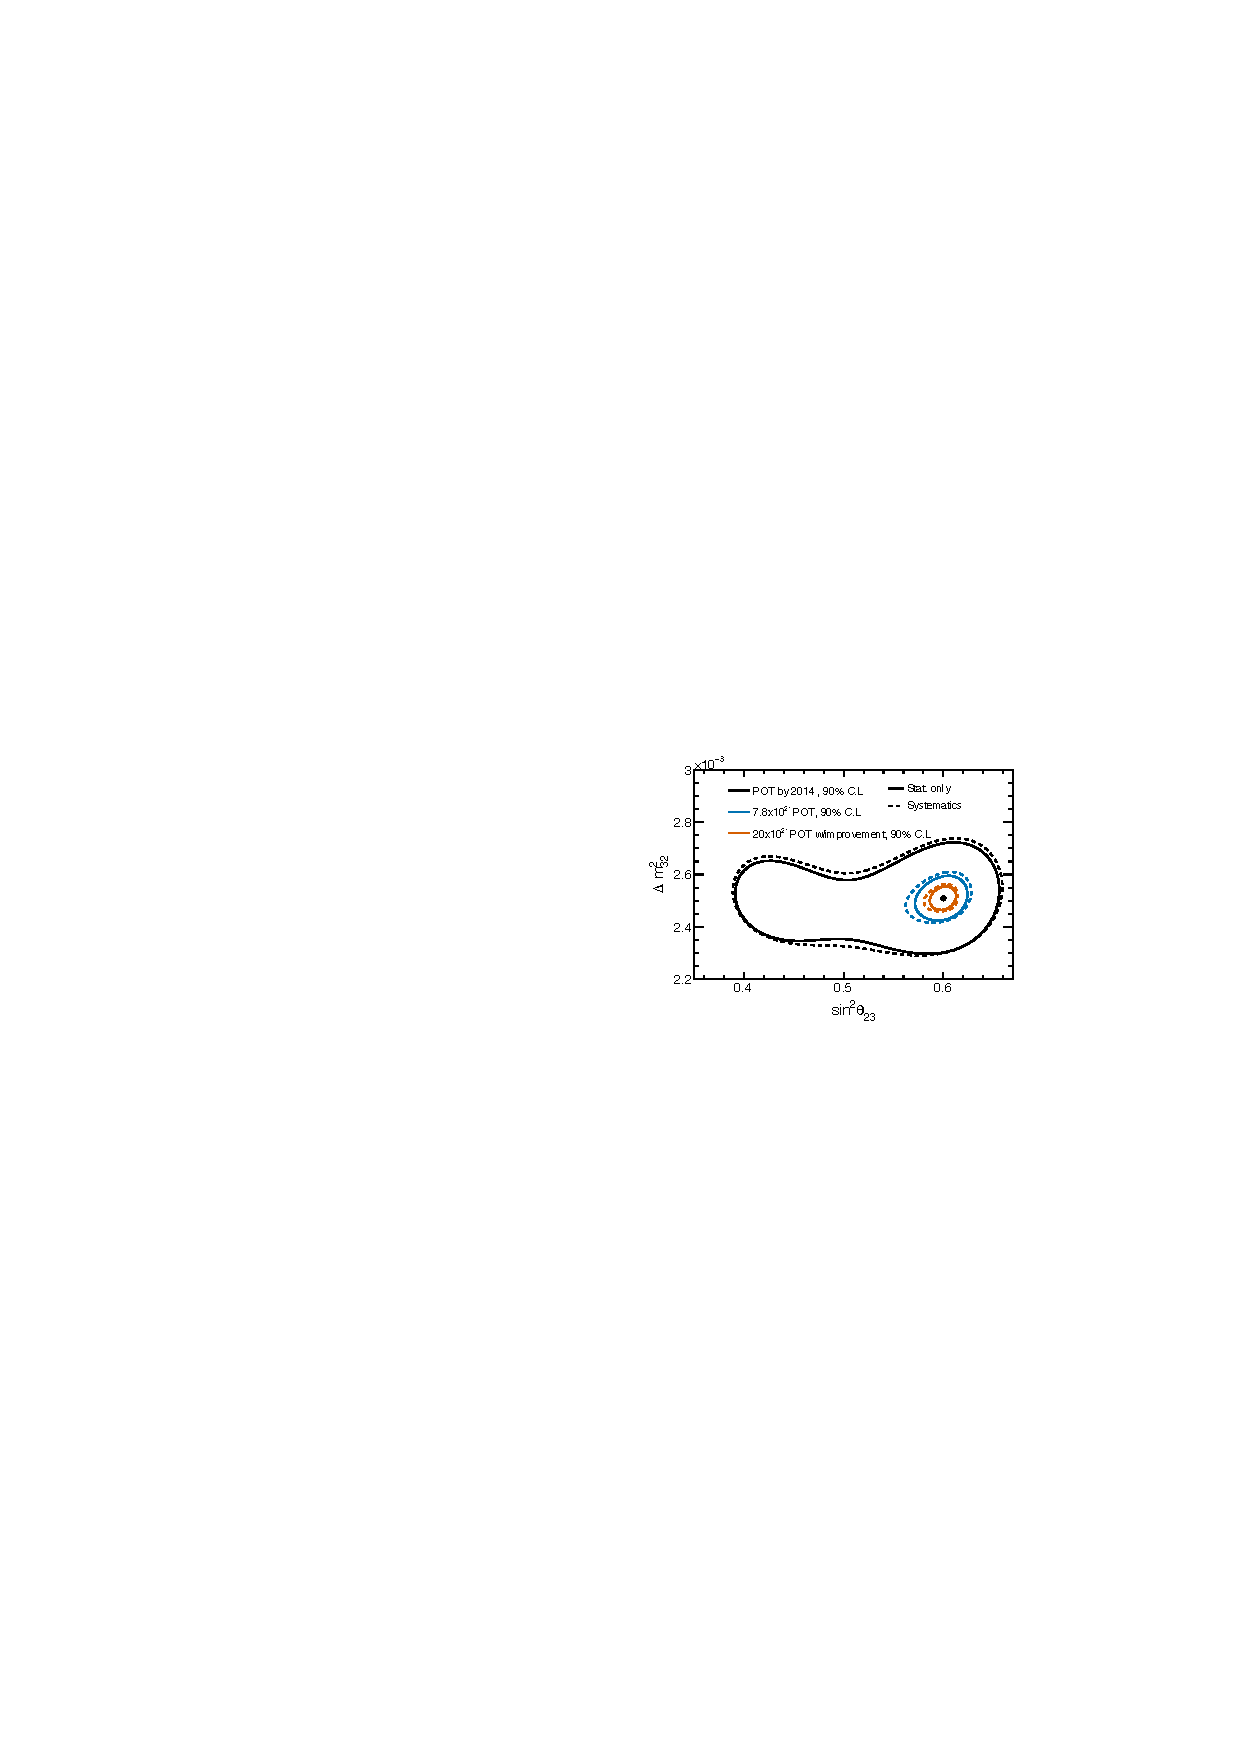
\includegraphics[width=8cm]{figures/t2kpre_t23dm32_point2_wreactorthrow.pdf}
\caption{\label{fig:t2k2th23} Expected improvements on the 90\% C.L. sensitivity to $\Delta m^2_{32}$ and $\sin^2\theta_{23}$
for T2K and T2K-II assuming \stt=0.5 (left) and \stt=0.6 (right).~\cite{Abe:2016tez}.}
\end{center}
\end{figure}

The main goal of \nova is instead to profit of the longer baseline with respect to T2K to determine the mass ordering. 

%The advantage of the longer baseline is shown in Fig.~\ref{fig:novaellipse} in which the appearance probability for \nue and \nueb is shown for different values of \dcp in the two mass ordering cases. The elliptical shapes are due to the fact that different values of \dcp lead to enhance one appearance probability  reducing the other while the separation between the two ellipses is due to the fact that the normal ordering increase the \nue appearance probability for all the values of \dcp while the \nueb appearance probability is increased in the inverted ordering scenario.
%
%
%\begin{figure} [h!]
%\begin{center}
%%add plot!!!
%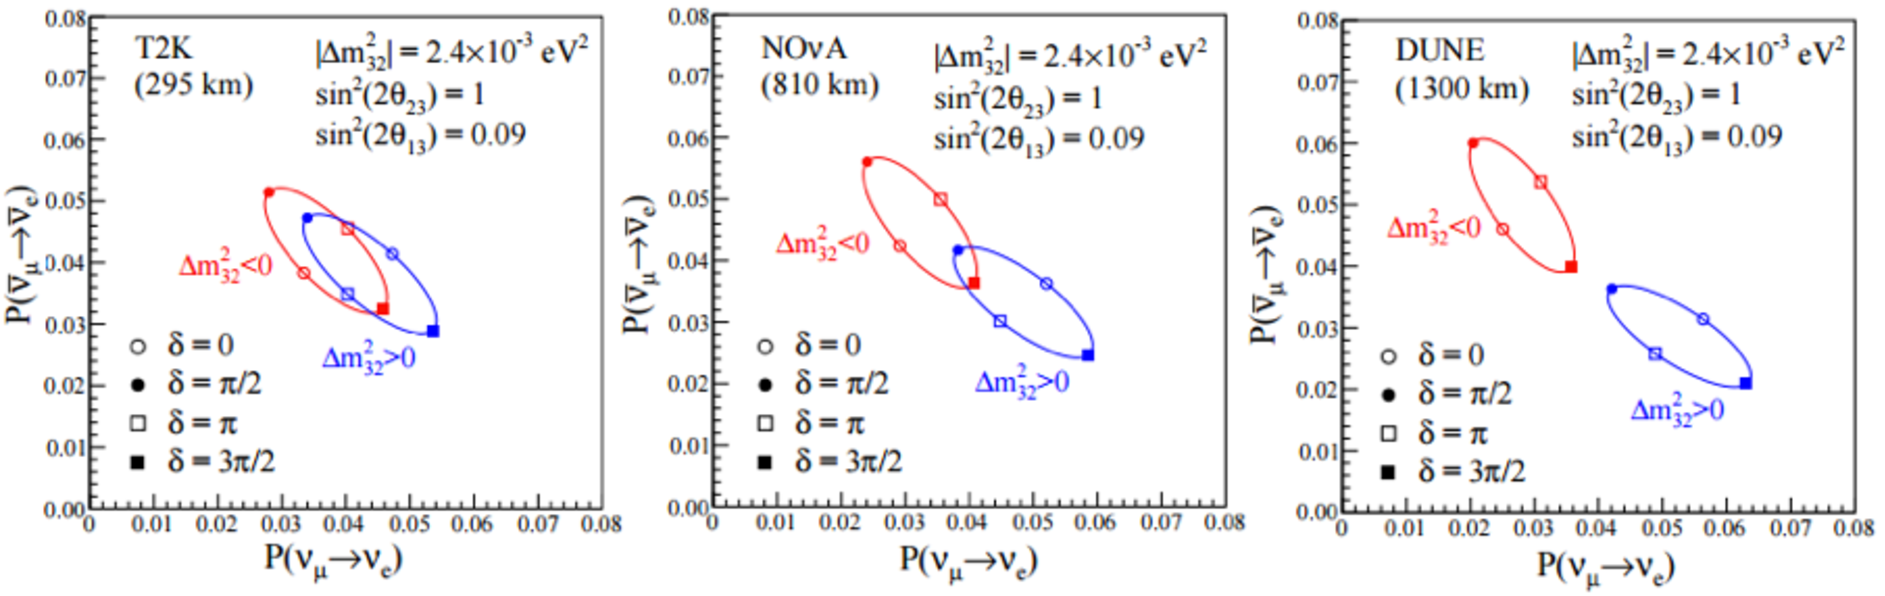
\includegraphics[width=8cm]{figures/t2k_nova_dune_ellipse.pdf}
%\caption{\label{fig:novaellipse} Equiprobabilities curves for T2K, \nova, and DUNE baseline}
%\end{center}
%\end{figure}
Also in the case of \nova the capability of measuring the ordering strongly depends on the combination of matter effects with \dcp. This is true for any experiment in which the baseline is not long enough to fully solve the degeneracies in the appearance probabilities due to the interplay between matter effects and \dcp. 
%Unless the baseline is long enough to solve the degeneracy as it is the case for the proposed \dune experiment, the capability of measuring the mass ordering depends on the combination of the matter effects with \dcp. 
%The appearance probability of \nue and \nueb is measured with a certain precision depending on the experiment. The mass ordering is determined if the combination of the two probabilities unambiguously identifies one solution. In the case of \nova the capability of the experiment to determine the mass ordering strongly depends on the values of \dcp and of the ordering. 
For example, if the mass ordering is normal then \nova will have a chance to measure it if \dcp is close to $-\pi/2$ while if \dcp is close to $\pi/2$ the degeneracy with the solution inverted ordering and $\dcp=-\pi/2$ would not be solved and a determination of the mass ordering would be impossible. In case the mass ordering is inverted, the situation is opposite: it will be possible to determine the mass ordering if \dcp=$\pi/2$ while there is no sensitivity for \dcp=$-\pi/2$. This is clearly reflected in the expected sensitivity of \nova to the mass ordering with $36\times10^{20}$~\pot, shown in Fig.~\ref{fig:novasensi}.
In the two lucky cases of $\dcp=-\pi/2$ and NO or $\dcp=\pi/2$ and IO the mass ordering will be determined at roughly $3\sigma$ by \nova while in the other cases the degeneracies among oscillation parameters will wash out the sensitivity of the experiment to the mass ordering. For these cases the combination with T2K and its different baseline will help at some level to solve the degeneracies but the sensitivity will not be enough to claim a measurement of the mass ordering with the current long-baseline experiments. The sensitivity of \nova to \dcp with  $36\times10^{20}$~\pot is shown in Fig.~\ref{fig:novasensidcp}.


\begin{figure} [htbp!]
\begin{center}
%add plot!!!
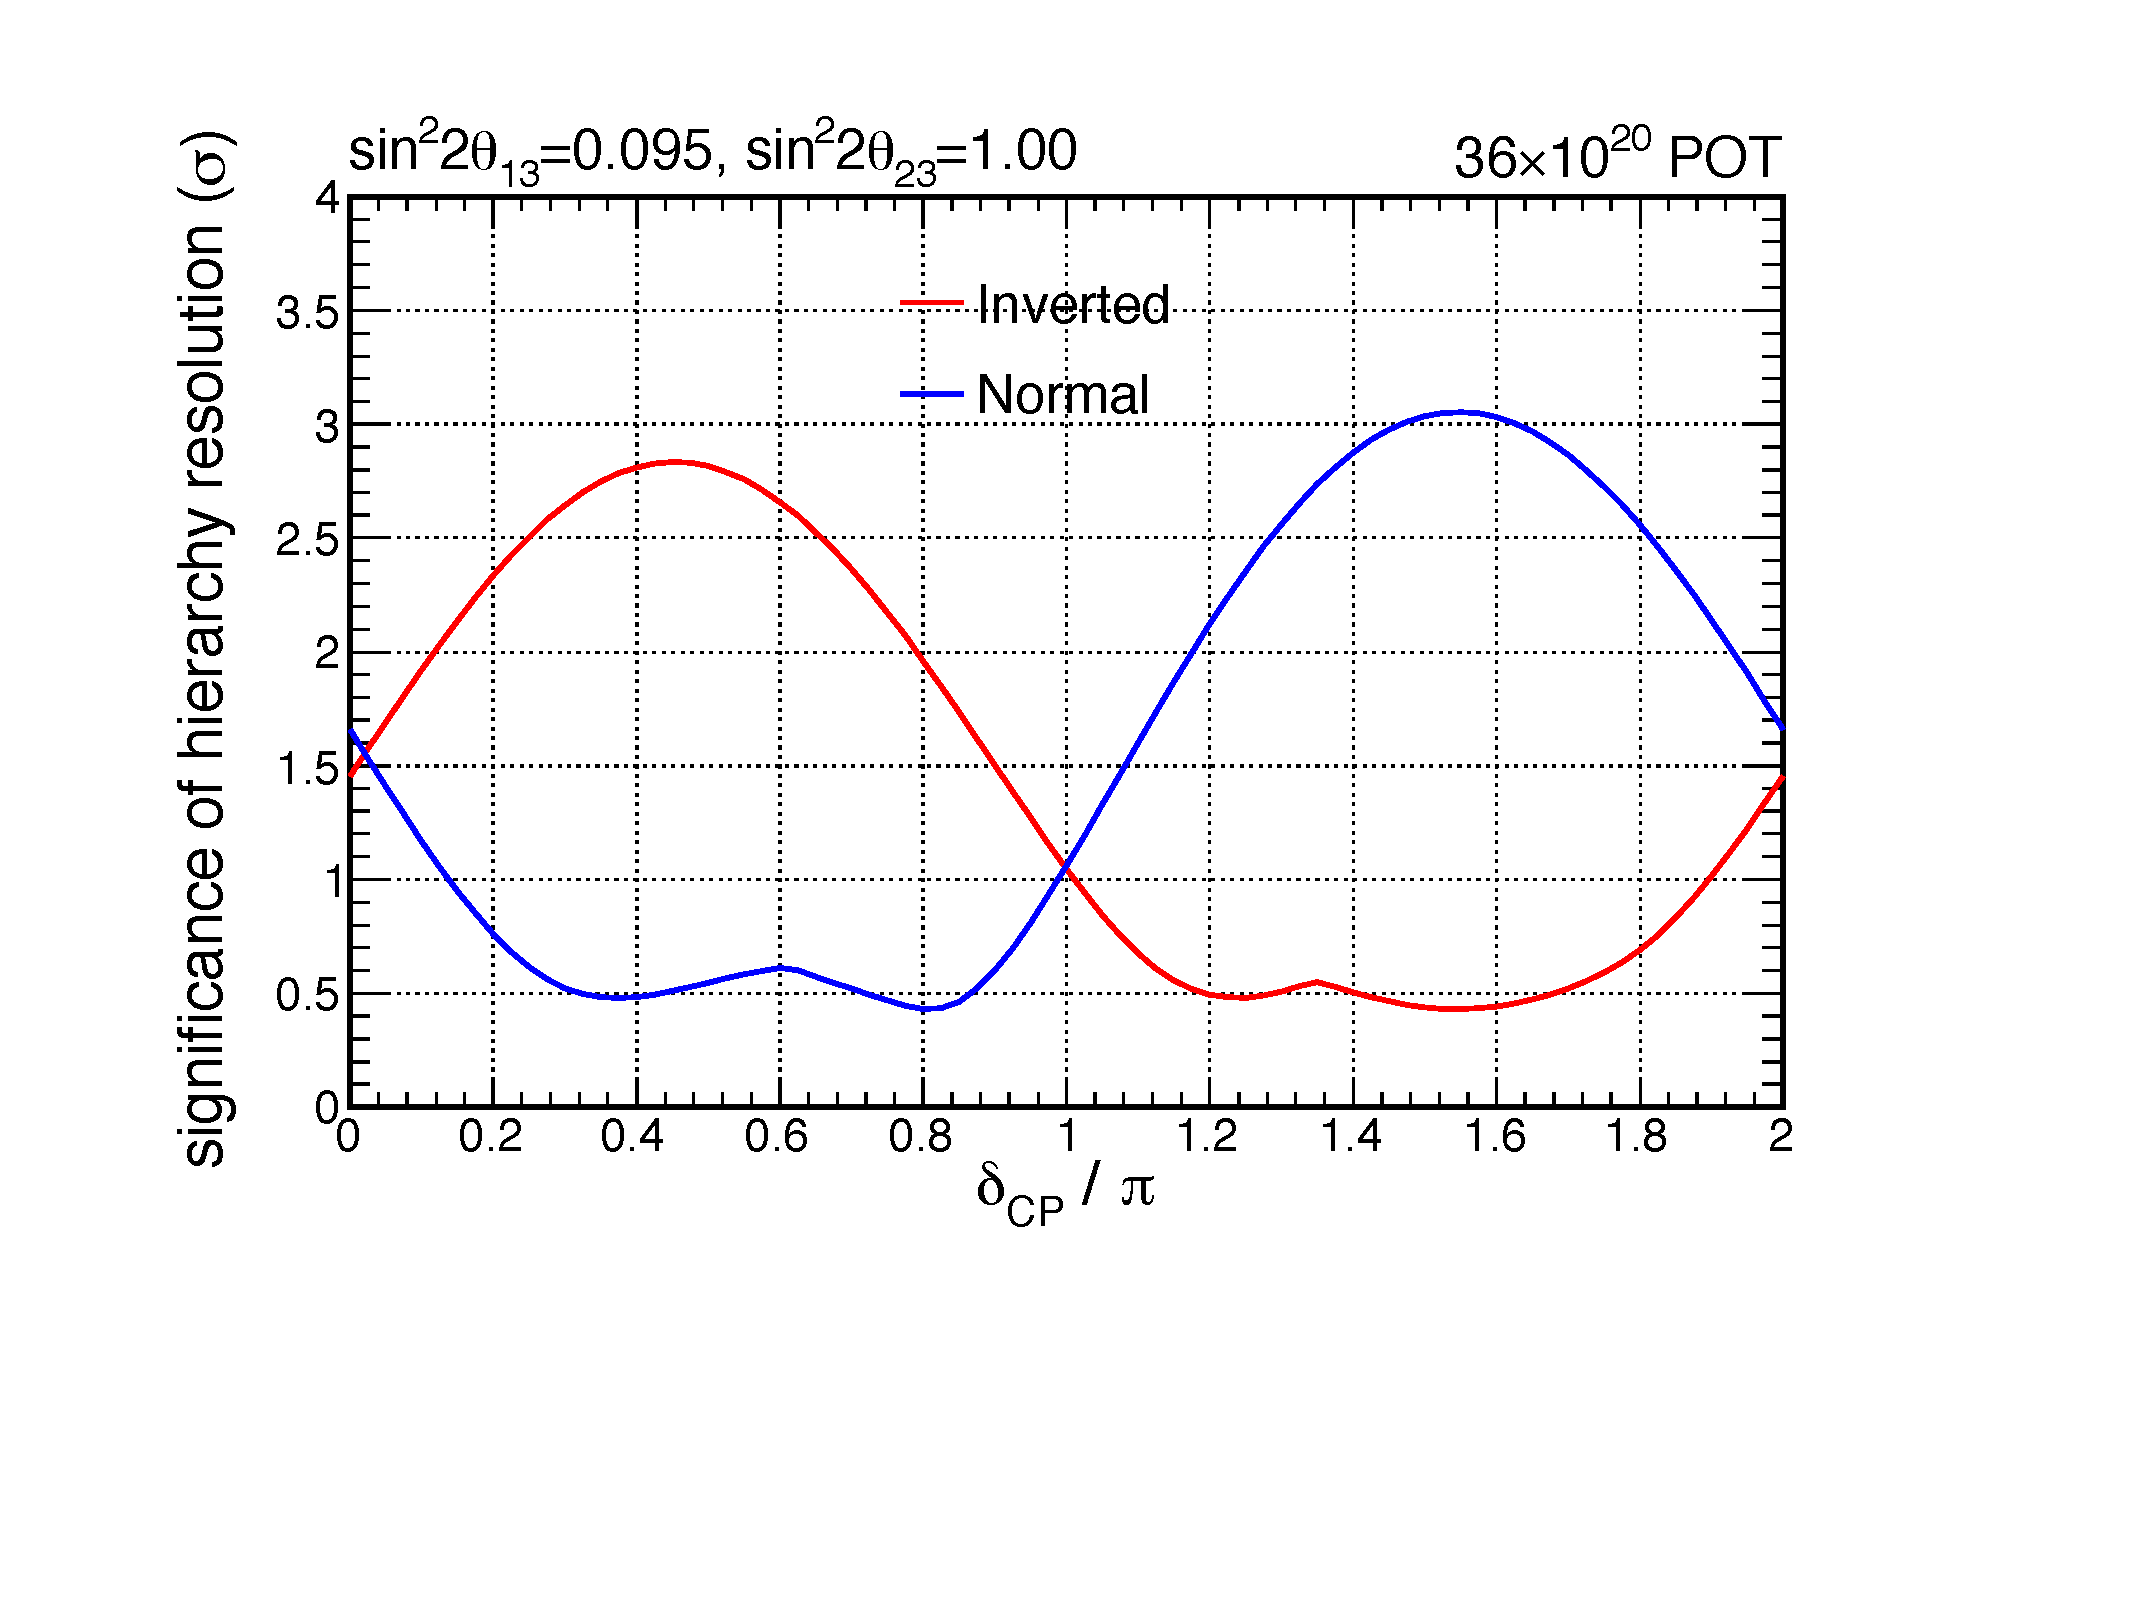
\includegraphics[width=8cm]{figures/nova_massordering.pdf}
\caption{\label{fig:novasensi} \nova sensitivity to the mass ordering with $36\times10^{20}$~\pot~\cite{messier2016}.}
\end{center}
\end{figure}

\begin{figure} [htbp!]
\begin{center}
%add plot!!!
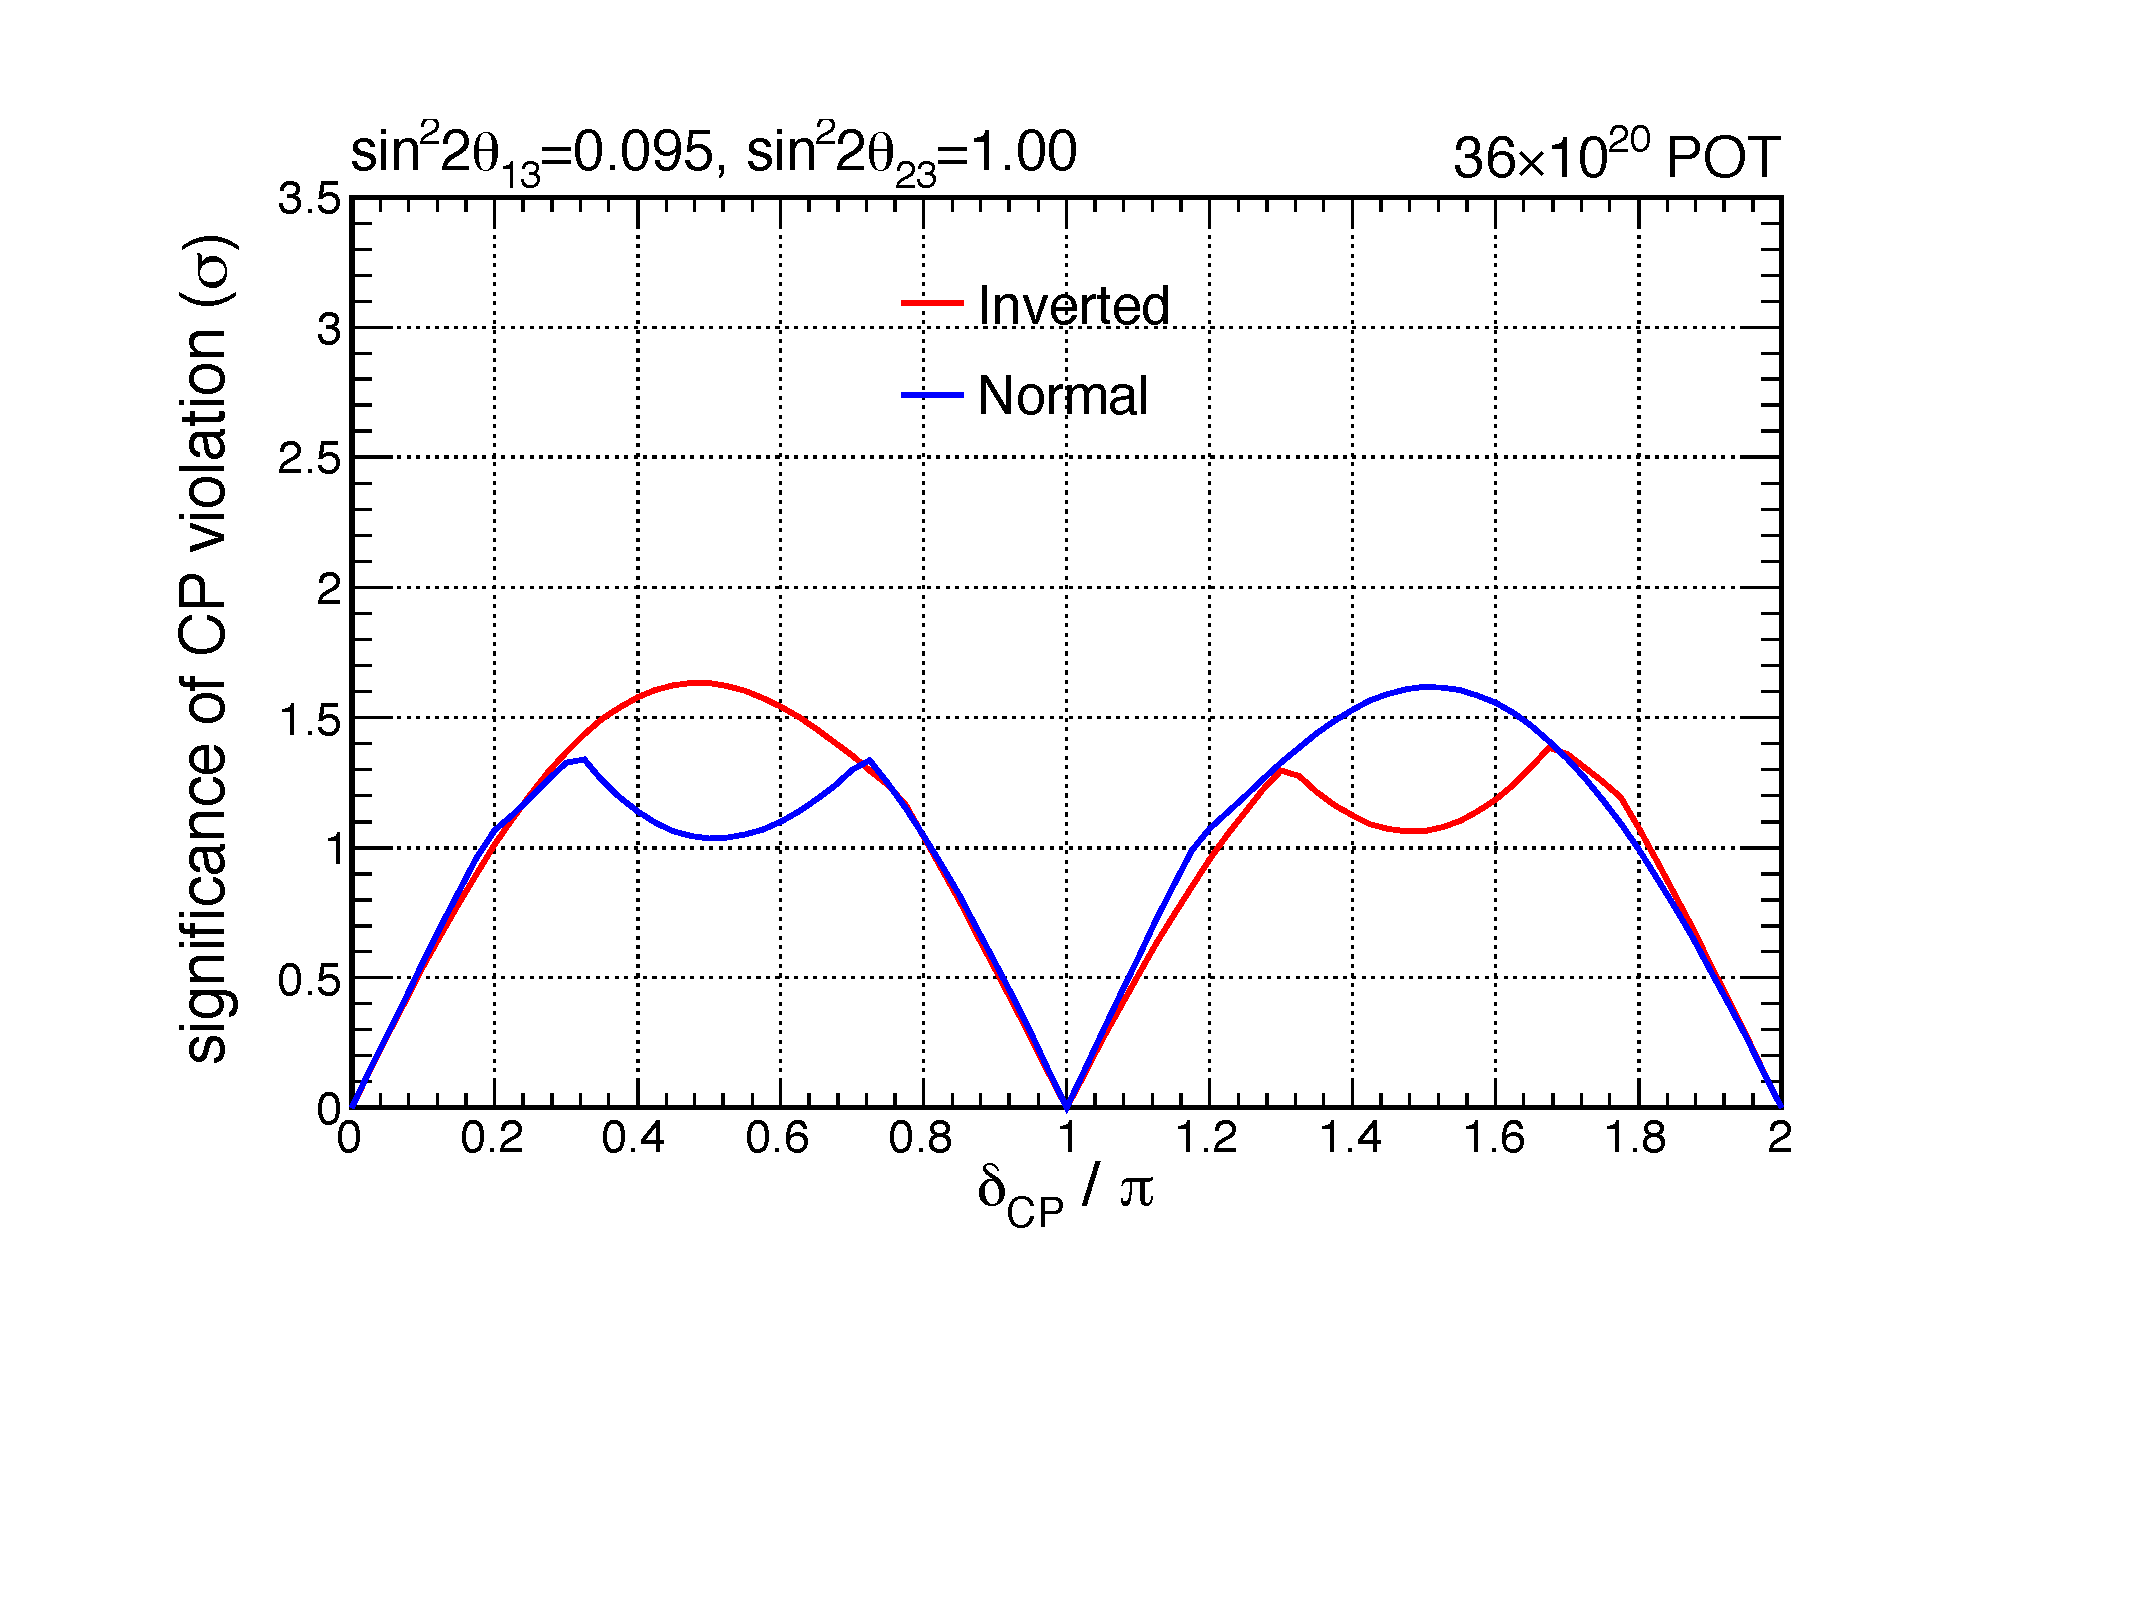
\includegraphics[width=8cm]{figures/nova_dcpmessier.pdf}
\caption{\label{fig:novasensidcp} \nova sensitivity to \dcp with $36\times10^{20}$~\pot~\cite{messier2016}.}
\end{center}
\end{figure}



%NOVA MH sensitivity (depends on delta)

%(where do we add  SK ?)

%increased sensitivity to theta23


\subsection{Next generation of non-accelerator based experiments}

While the best technique to measure CP violation in the leptonic sector is by using long-baseline accelerators, measuring \nue and \nueb appearance probabilities, different techniques can be used for the measurement of the mass ordering.
It is generally the case that to measure the mass ordering the experiment must be sensitive either to three neutrino effects or to matter effects. Indeed, we have shown that in most of the experiments the leading order vacuum oscillation probability have the form $P(\nu_\alpha \rightarrow \nu_\beta) = \sin^2 2 \theta sin^2 (\frac{\Delta m^2 L}{4E})$ which is insensitive to the sign of $\Delta m^2$. 

As we have seen in Sect.~\ref{sec:futuret2knova}, the mass ordering can be measured by exploiting the matter effects in long-baseline experiments as for example \nova and can be measured for any value of \dcp by doing experiments with a longer baseline such as the proposed DUNE experiment that will be described in the next section. Other possibilities to measure the mass ordering are provided by the exploitation of matter effects using atmospheric neutrinos (ORCA, PINGU, INO, Hyper-Kamiokande) or by testing the interference between \dmsq and \dmsqtwo. 

The latter idea is exploited by the JUNO experiment~\cite{An:2015jdp} that foreseen a 20~kton liquid scintillator detector to be installed at a distance of 53~km from some nuclear reactors in China producing \nueb. 
Anti-neutrinos are produced in nuclear reactors with energies in the range from 1 to 8~MeV. The first oscillation maximum, driven by \dmsqso, occurs at distances from the reactor core of roughly 100~km while the oscillation maximum driven by the atmospheric oscillation mass-splitting \dmsq occurs at distances of roughly 2~km. As we have seen in the previous sections, the first effect is exploited by KamLAND to measure \thsol and \dmsqso while the later is exploited by Daya Bay, RENO, and Double Chooz to measure \thint. 

At the longer of these baselines, the atmospheric-driven oscillations also manifests as a small and rapid oscillation superimposed to the slower solar-driven oscillations. The relative phase of these oscillations depends on the relative size of \dmsq and \dmsqtwo and so on the mass ordering. This can be seen from the \nueb survival probability that at distances of $\sim55~km$ can be written as:

\begin{equation}
P(\bar{\nu}_e \rightarrow \bar{\nu}_e) = 1 - \cos^4 \theta_{13} \sin^2 2 \theta_{12}  \sin ^2 \Delta_{21}
- \sin^2 2 \theta_{13} (\cos^2  \theta_{12} sin^2 \Delta_{31} + \sin^2  \theta_{12}  \sin^2 \Delta_{32} ),
\end{equation} 
where $\Delta_{ij}= \Delta m^2_{ij} L/(4E)$.

The spectrum is strongly distorted by the neutrino oscillations: a large deficit of \nueb is expected, dominated by the solar parameters \thsol and \dmsqso as shown on Fig.~\ref{fig:junospectrum} where the effect due to the atmospheric mass-squared difference is also visible, manifesting itself as multiple cycles (fast oscillations) in the reactor energy spectrum. 
Changing the sign of \dmsq shifts the period and the phase of these oscillations by 180 degrees and this effect is exploited to measure the mass ordering.
%The position of these cycles depends on the ordering as can be understood from the fact that for normal ordering $|\Delta m_{31}^2| > |\Delta m_{32}^2|$ while the opposite is the case for inverted ordering.


JUNO (Jiangmen Underground Neutrino Observatory) is a multi-purpose neutrino experiment with the main goal of determining the mass ordering will be a 20 kton liquid scintillator detector that will be installed at a distance of 53~km from two sites hosting nuclear plants in China, where a total of ten power plants will in operation by 2020. The detector will be located underground with an overburden of more than 700~m and it will be composed by a liquid scintillator spherical detector submerged into a water pool instrumented with PMTs acting as a shield from natural radioactivity. On the top of the water pool a tracking detector will also be installed to tag muons. 

In a liquid scintillator detector such as JUNO, neutrinos emitted by reactors are observed via the inverse $\beta$-decay already described in section~\ref{subsec:reactorflux}. 
%In this process a positron and a neutron are emitted, with the positron quickly depositing its energy, providing a prompt signal. The neutron is instead captured by a proton after few hundreds of $\mu s$. In the capture process a 2.2 MeV $\gamma$ is released, providing a delayed signal. The coincidence between prompt and delayed signals provides a distinctive signature of the antineutrino interaction.
However, in order to extract the MO information from the spectral distortion, an excellent energy resolution ($3\%/ \sqrt{E}$), a good understanding of the energy response (better than 1\%), and a large statistics ($>100k$ inverse beta decay events) are required.
 
\begin{figure} [h!]
\begin{center}
%add plot!!!
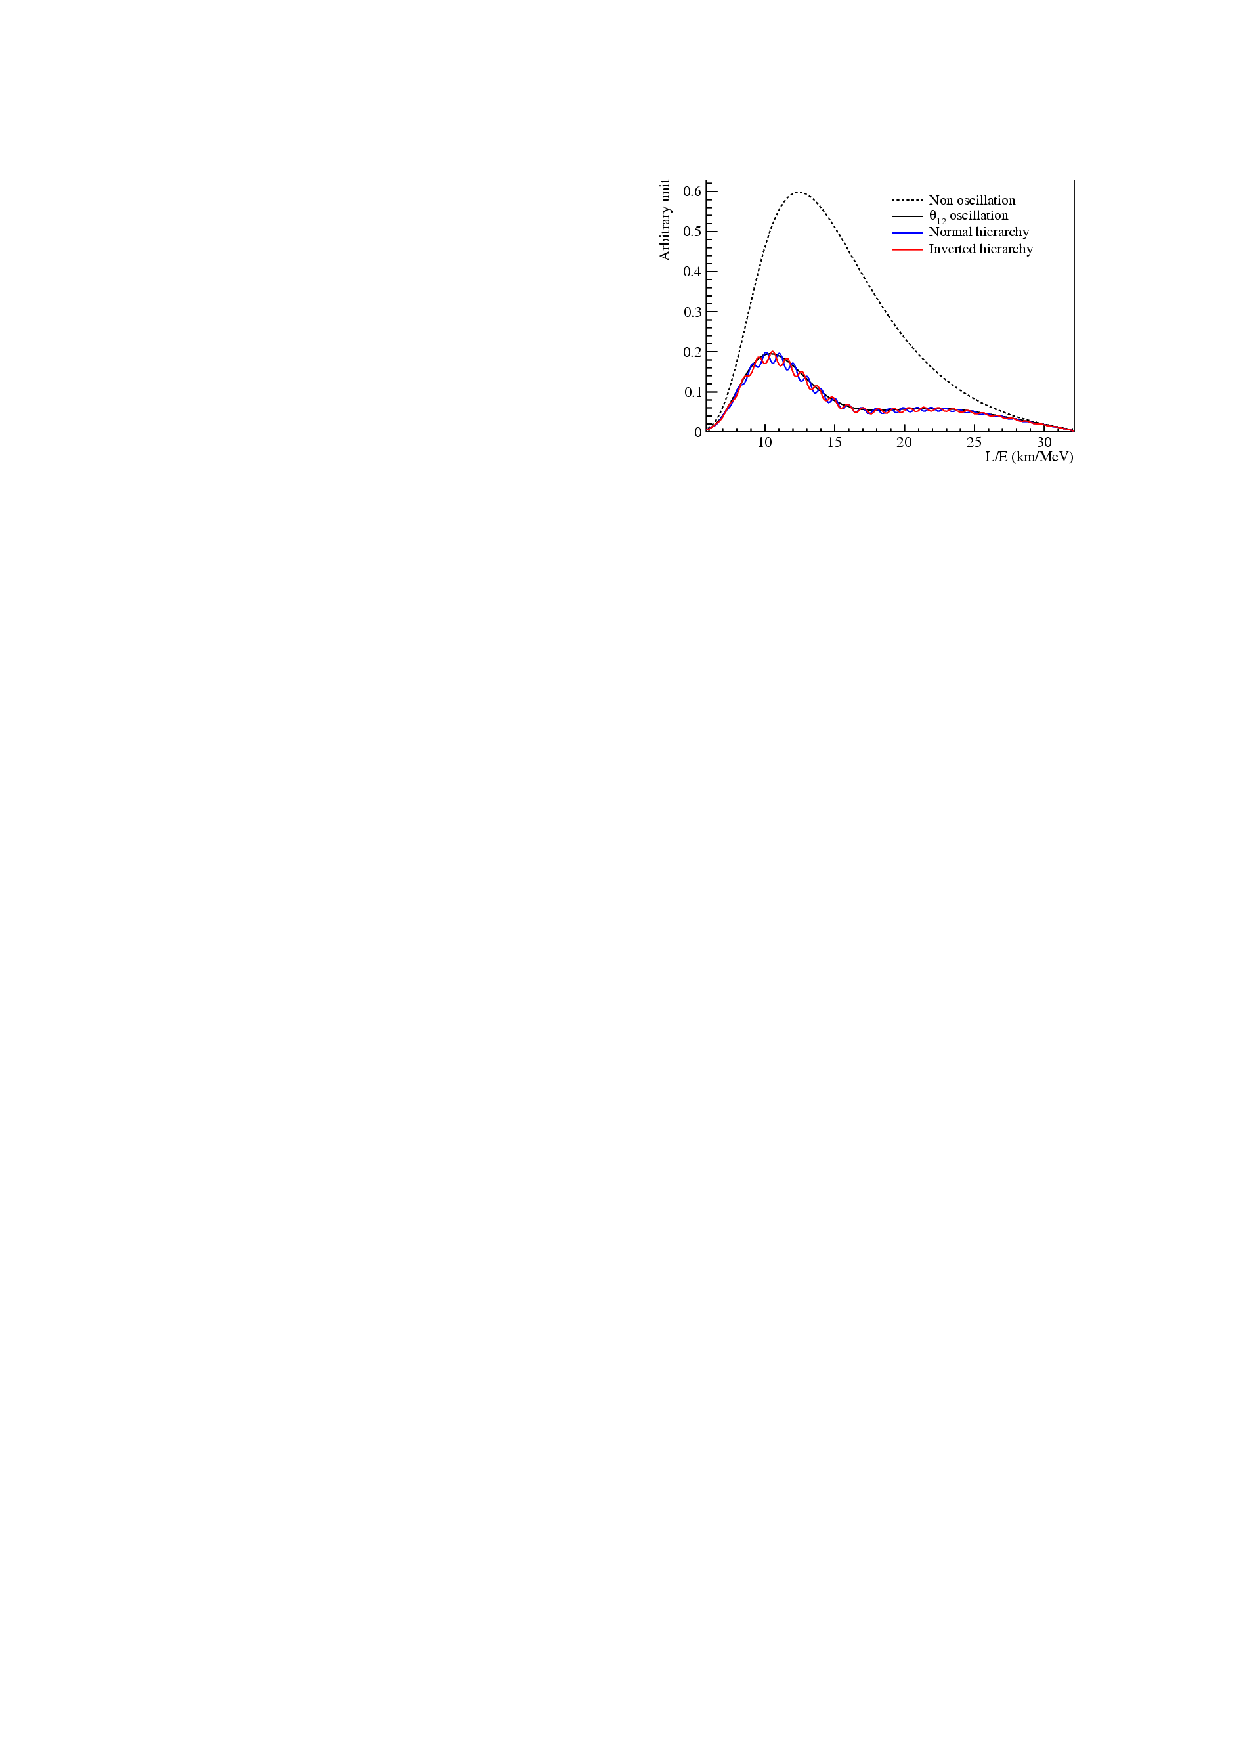
\includegraphics[width=8cm]{figures/JUNO_spectrum.pdf}
\caption{\label{fig:junospectrum} Shape difference of the reactor antineutrino flux for the two mass ordering cases~\cite{An:2015jdp}.}
\end{center}
\end{figure}

Such a statistics will be obtained thanks to the large size of the JUNO detector while the required precision on the energy resolution and on the energy response will be more difficult to reach and requires important improvements with respect to what was reached for the Daya Bay experiment. Particularly it is required to have PMT photocathode coverage larger than 75\%, a PMT quantum efficiency larger than 35\% and an attenuation length of the liquid scintillator larger than 20~m at 430~nm. If these requirements are reached, JUNO expect a median sensitivity for the determination of the mass ordering of $3\sigma$ after six years of data taking. The sensitivity can be improved to $\sim4\sigma$ if the precision in the measurement of the atmospheric mass splitting in long baseline experiments will reach the 1\% level.
The impact of the energy resolution on the determination of the mass ordering is shown in Fig.~\ref{fig:junoeneres}.

\begin{figure} [htbp!]
\begin{center}
%add plot!!!
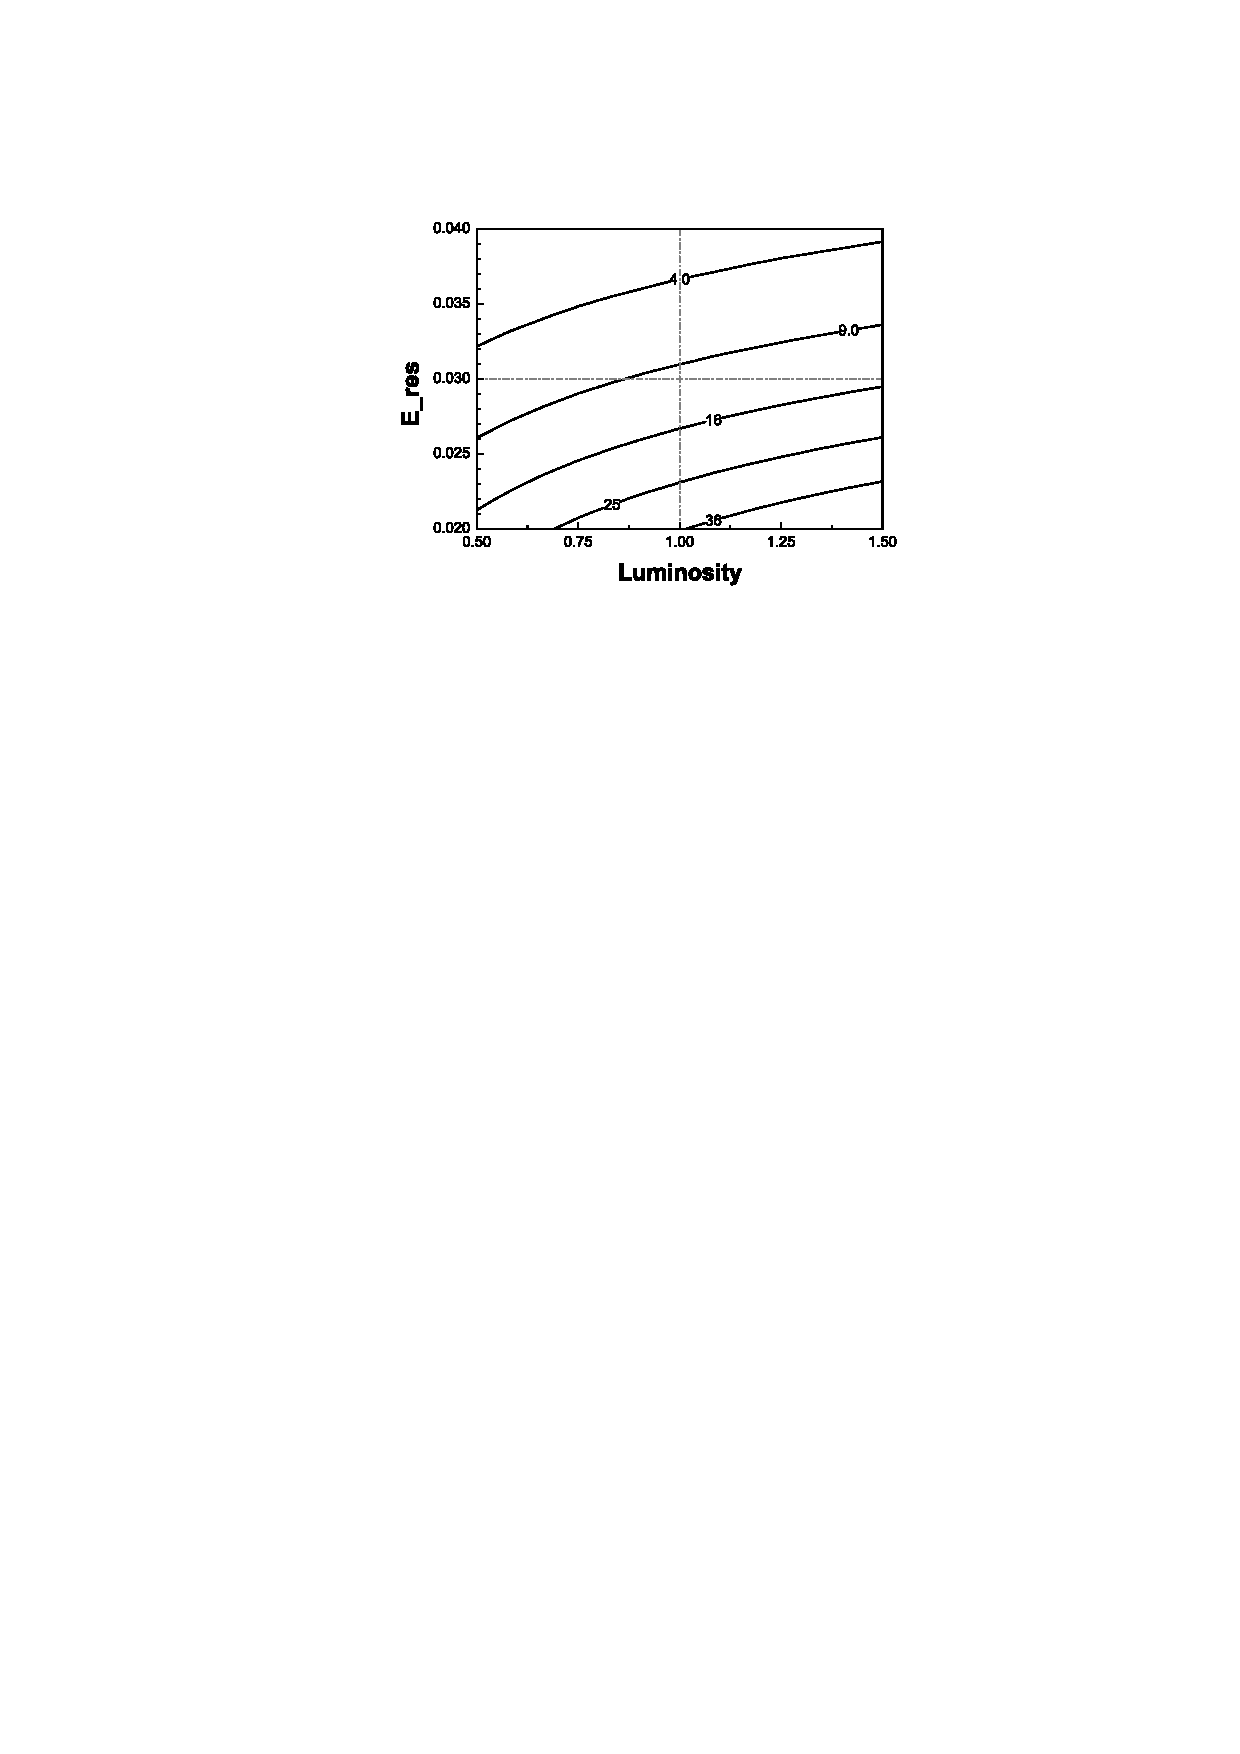
\includegraphics[width=8cm]{figures/juno_energyres.pdf}
\caption{\label{fig:junoeneres} The iso-$\Delta\chi^2$ contour plot to determine the mass ordering as the function of the event statistics (luminosity) and the energy resolution. The vertical dash-dotted line represent the nominal running of six years with 80\% signal efficiency and a 3\% energy resolution~\cite{An:2015jdp}.}
\end{center}
\end{figure}


Besides the determination of the mass ordering, JUNO will perform several precise measurements of the neutrino mixing parameters. While the precision of \thint will still be dominated by Daya Bay thanks to its shorter baseline, the huge number of events collected by JUNO, will allow to dramatically improve the uncertainties on the solar parameters, \thsol and \dmsqso. As we have seen in Sect.~\ref{sec:solar} those parameters are currently measured by KamLAND (dominating the \dmsqso measurement) and solar neutrino experiments (dominating the \thsol measurement) with uncertainties of the order of 2-4\%. JUNO will be able to reduce the uncertainties on these parameters well below 1\%, allowing precise tests of the unitarity of the lepton mixing matrix.

In addition JUNO will also observe galactic supernovae burst, collect $\sim5000$ inverse beta decay, 2000 elastic neutrino-proton scattering and 300 elastic neutrino-electron scattering for a SN explosion at a distance of 10 kpc. The time evolution, energy spectra and flavor contents of SN neutrino can be used to investigate the explosion mechanism. Also neutrinos from the diffuse supernova neutrino background might be observed by JUNO. Finally JUNO will be able to perform precise measurements of the flux of solar neutrinos from $^8$B and $^7$Be thanks to the high light yield, exceptional energy resolution, and  low threshold. The statistics collected in JUNO will allow to help solving the solar composition problem, and probe the transition region between the vacuum-dominated and MSW-dominated neutrino oscillations. 

An alternative technique for the measurement of the mass ordering has been proposed using the matter effects on the propagation of atmospheric neutrinos~\cite{razzaque}.
The mass ordering would be measured by exploiting the different oscillation probabilities due to matter effects for neutrinos crossing the Earth. The oscillation probabilities, or oscillograms, for the two mass orderings are shown in Fig.~\ref{fig:orcaoscprob} as a function of the energy and the cosine of the zenithal angle $\theta_z$.
The qualitative features of these oscillograms can be understood as follows. The Earth density can be simply modelled as the mantle with an almost constant density of about 4 g/cm$^3$ above a radius of 3000 km and a core density of about 7 g/cm$^3$ below that radius.
The most prominent features of these oscillograms are the $\nu_\mu \rightarrow \nu_e$ MSW resonance in the mantle for E $\simeq$ 7 GeV, visible at a $\cos \theta_z \simeq -0.8$, where $\theta_z$ is the zenithal angle, and  the MSW resonance in the core for 
  E $\simeq$ 3 GeV for $\cos \theta_z < -0.8$. As already explained, the resonance is present either in the neutrino channel for NO or in the antineutrino channel for IO. This resonance has a spectacular effect in the 
  $\nu_\mu \rightarrow \nu_e$ channel but also a large related impact in the $\nu_\mu \rightarrow \nu_\mu$ channel. The finer structure seen in the $\cos \theta_z < -0.8$ region is due to the parametric resonance effect~\cite{akhmedov}, related to the propagation of these neutrinos first in the mantle, then in the core and again in the mantle. 
  
The detectors based on the Cherenkov technique like ORCA, PINGU or Hyper-Kamiokande do not measure the charge of the of the lepton event-by-event but, by exploiting the different interaction probability between neutrinos and antineutrinos, a net asymmetry in the combined ($\nu+\nub$) event rate for \nue and \num can be observed. However the effect is strongly diluted. Smearing of the reconstructed energy and angle dilute this effect even more. Once the atmospheric neutrino fluxes and the neutrino-nucleon cross-section are taken into account, bidimensional plots of event rates as a function of neutrino energy and zenith angle are built as shown in Fig.~\ref{fig:orcaasym}. Although the asymmetry is partially washed out, there is still a certain sensitivity to the mass ordering. 

These experiments intend to instrument with a dense array of PMTs large volumes of ice in the Antarctica (PINGU) or water in the Mediterranean sea (ORCA) to observe through the Cherenkov effect the muon track or the electromagnetic showers produced by \num and \nue interactions in the medium. The technique is similar to the one used by ICECUBE and ANTARES to observe high energy neutrinos produced by cosmic rays but, in order to improve the energy and direction reconstruction, a much denser arrays of PMTs will be built, at the price of instrumenting a smaller area of water or ice. Indeed, one of the challenges of these experiments is to reach an energy threshold around 5 GeV, which is considerably lower than the 15 GeV obtained at present even for the IceCube DeepCore denser instrumented volume. This requires to arrange the PMTs at close distance, around 10m. Moreover, another challenge is to control the systematic uncertainties related to the reconstruction of the energy and the momentum.   

\begin{figure} [htbp!]
\begin{center}
%add plot!!!
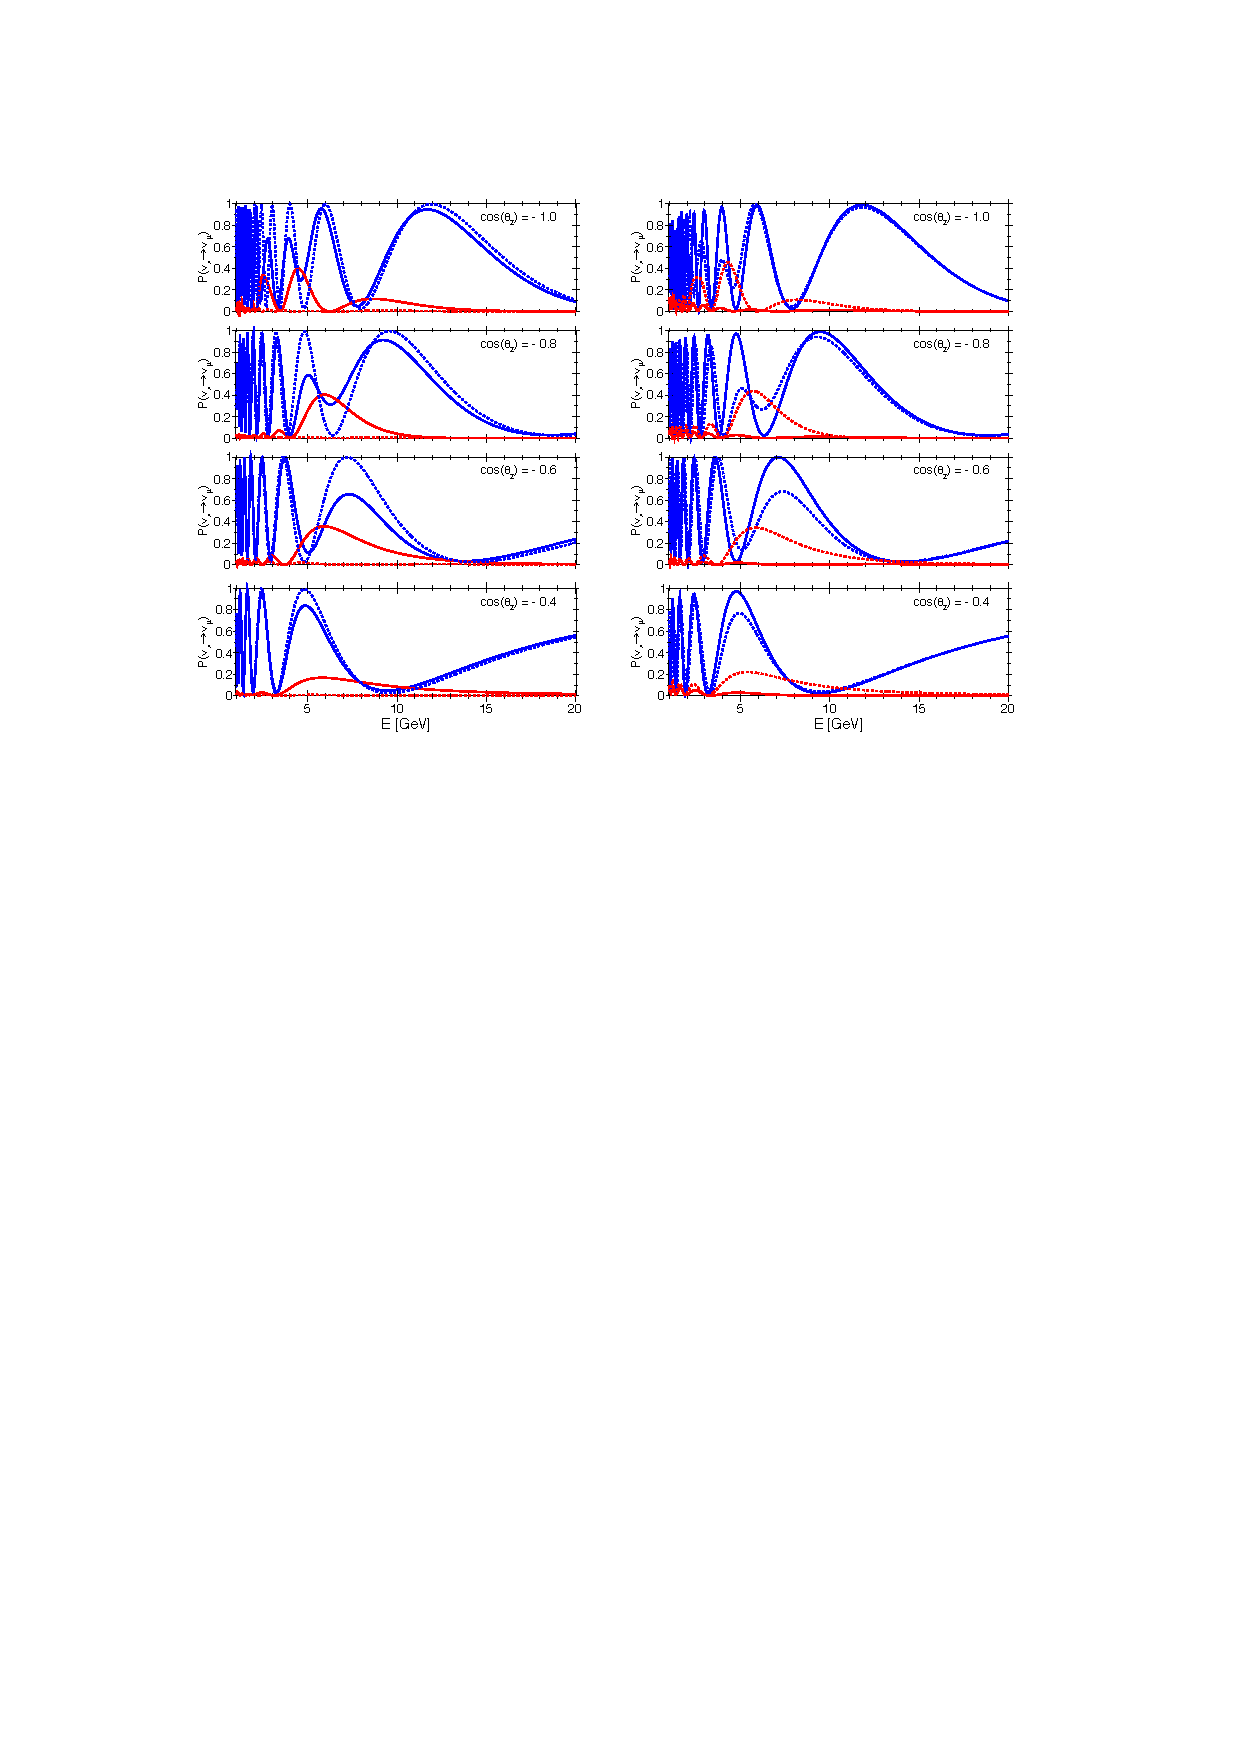
\includegraphics[width=12cm]{figures/orca_oscprob.pdf}
\caption{\label{fig:orcaoscprob} Oscillation probabilities for $\num \rightarrow \num$ (blue lines)  and $\nue \rightarrow \num$ (red lines) for different zenith angles. The solid (dashed) lines are for NO (IO)~\cite{Akhmedov:2012ah}.}
\end{center}
\end{figure}


%It should be noticed here that the smearing on tracks crossing the ice is larger than the one suffered by tracks crossing the water thus giving some advantages in terms of sensitivity to mass ordering to ORCA.

\begin{figure} [htbp!]
\begin{center}
%add plot!!!
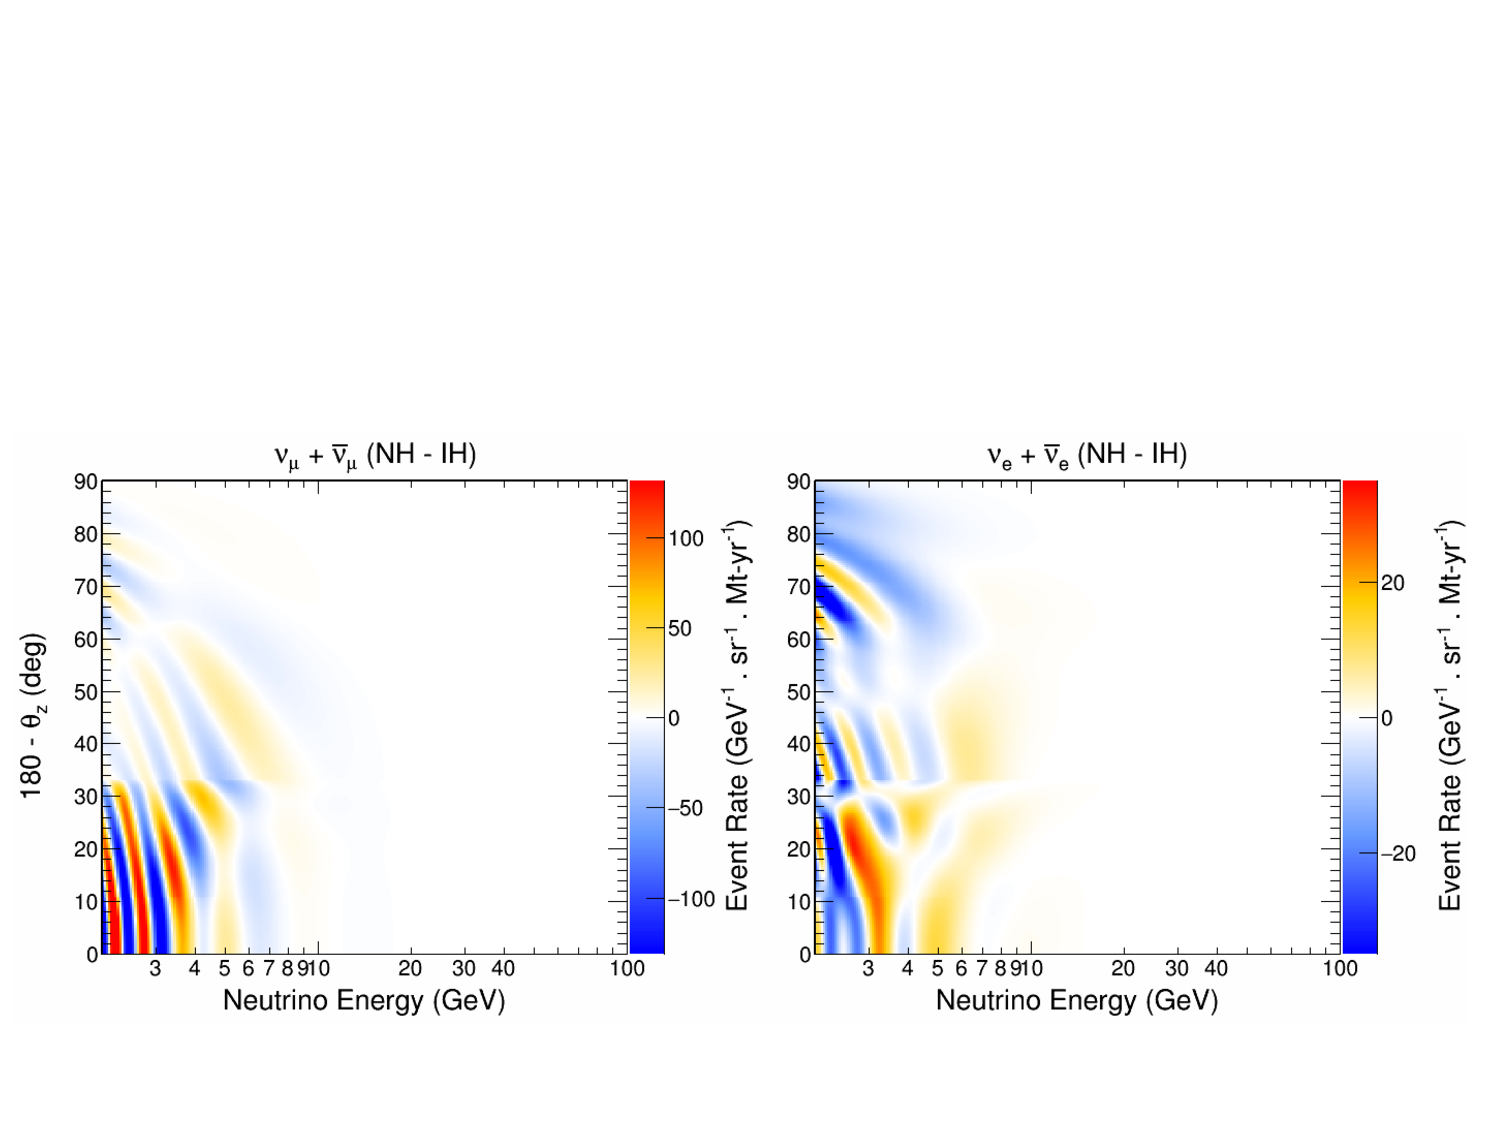
\includegraphics[width=12cm]{figures/orca_true2d.pdf}
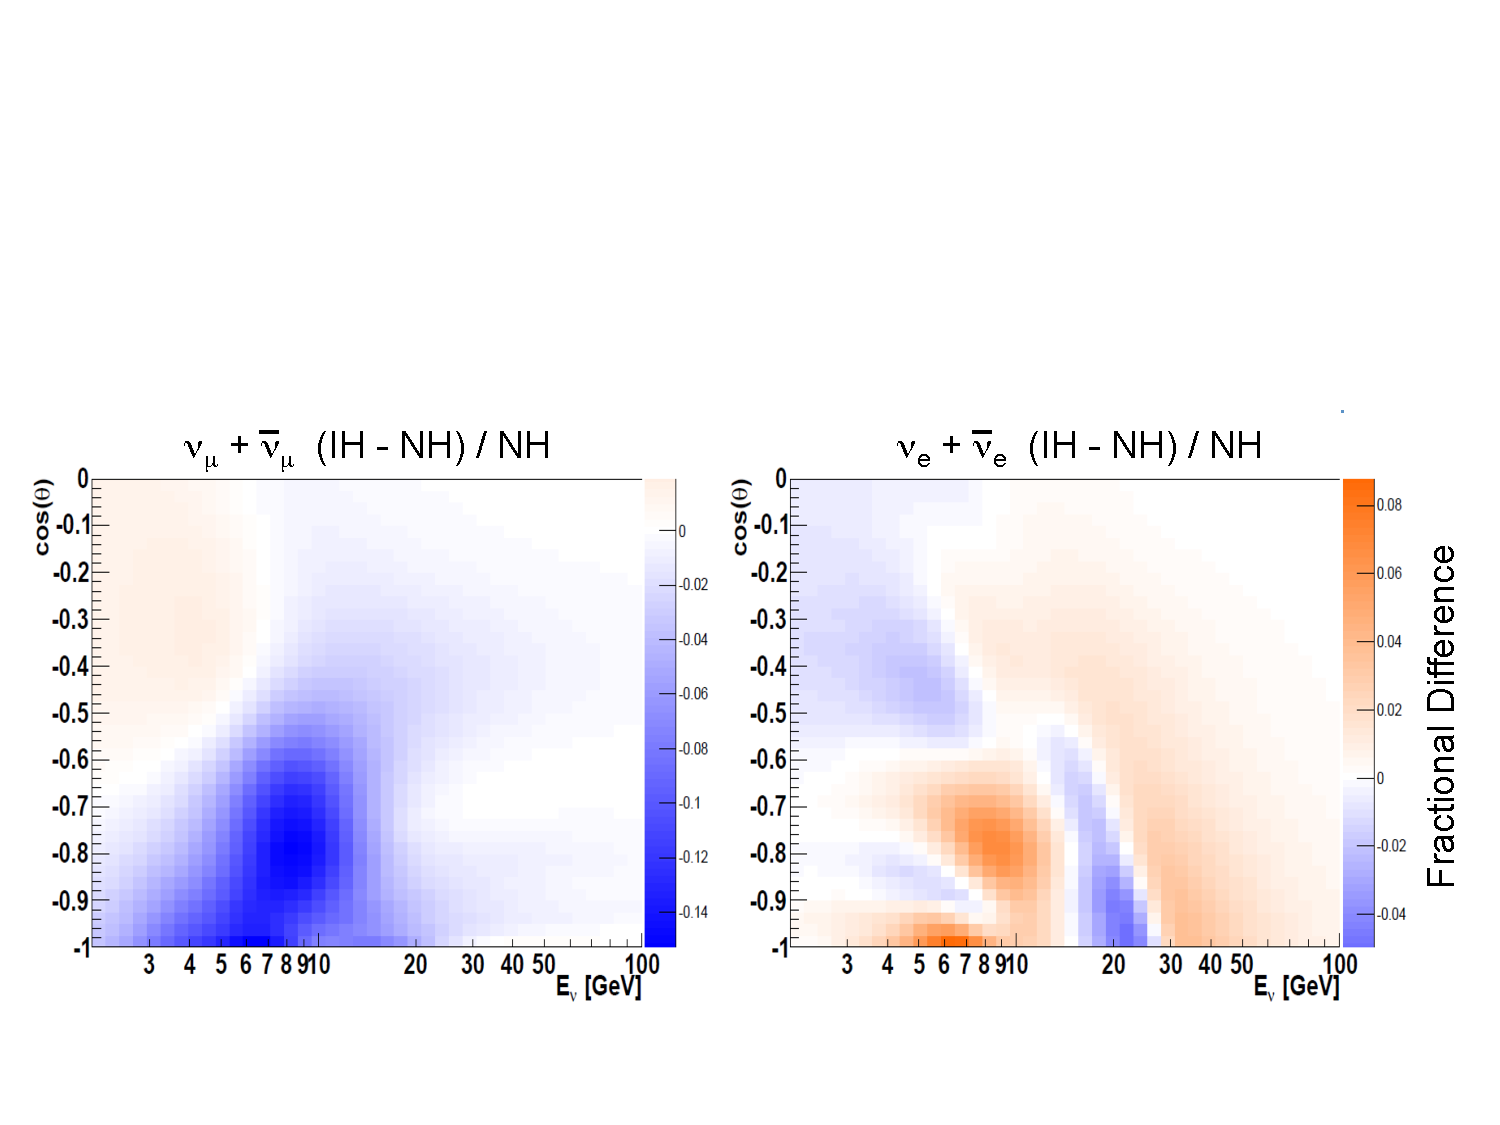
\includegraphics[width=12cm]{figures/orca_smear2d.pdf}
\caption{\label{fig:orcaasym} Asymmetry as a function of neutrino energy and zenith angle for \num (left) and \nue (right) in ORCA. On the bottom plots a 25\% smearing on the energy and angle reconstruction is applied.}
\end{center}
\end{figure}

In ORCA two categories of events are reconstructed: tracks produced by muons in \num charged current interactions and showers produced by neutral current interactions or \nue. Both contribute to the measurement of the mass ordering. The sensitivity mainly depends on the capability of reconstructing the energy and the angle of the incident neutrino from the observation of a shower or a track on the PMTs. The resolution depends on the spacing between the PMTs and, once the total number of PMTs is fixed, the optimal vertical spacing is 9~m. 

Assuming this configuration, the sensitivity of ORCA to the mass ordering after three years of run is shown in Fig.~\ref{fig:orcasensi}. The sensitivity depends on other PMNS oscillation parameters, in particular \thatm and \dcp but in general a sensitivity of $\sim3\sigma$ will be obtained. Similar results will be reached by PINGU after four years of running as shown in Fig.~\ref{fig:pingusensi}

\begin{figure} [htbp!]
\begin{center}
%add plot!!!
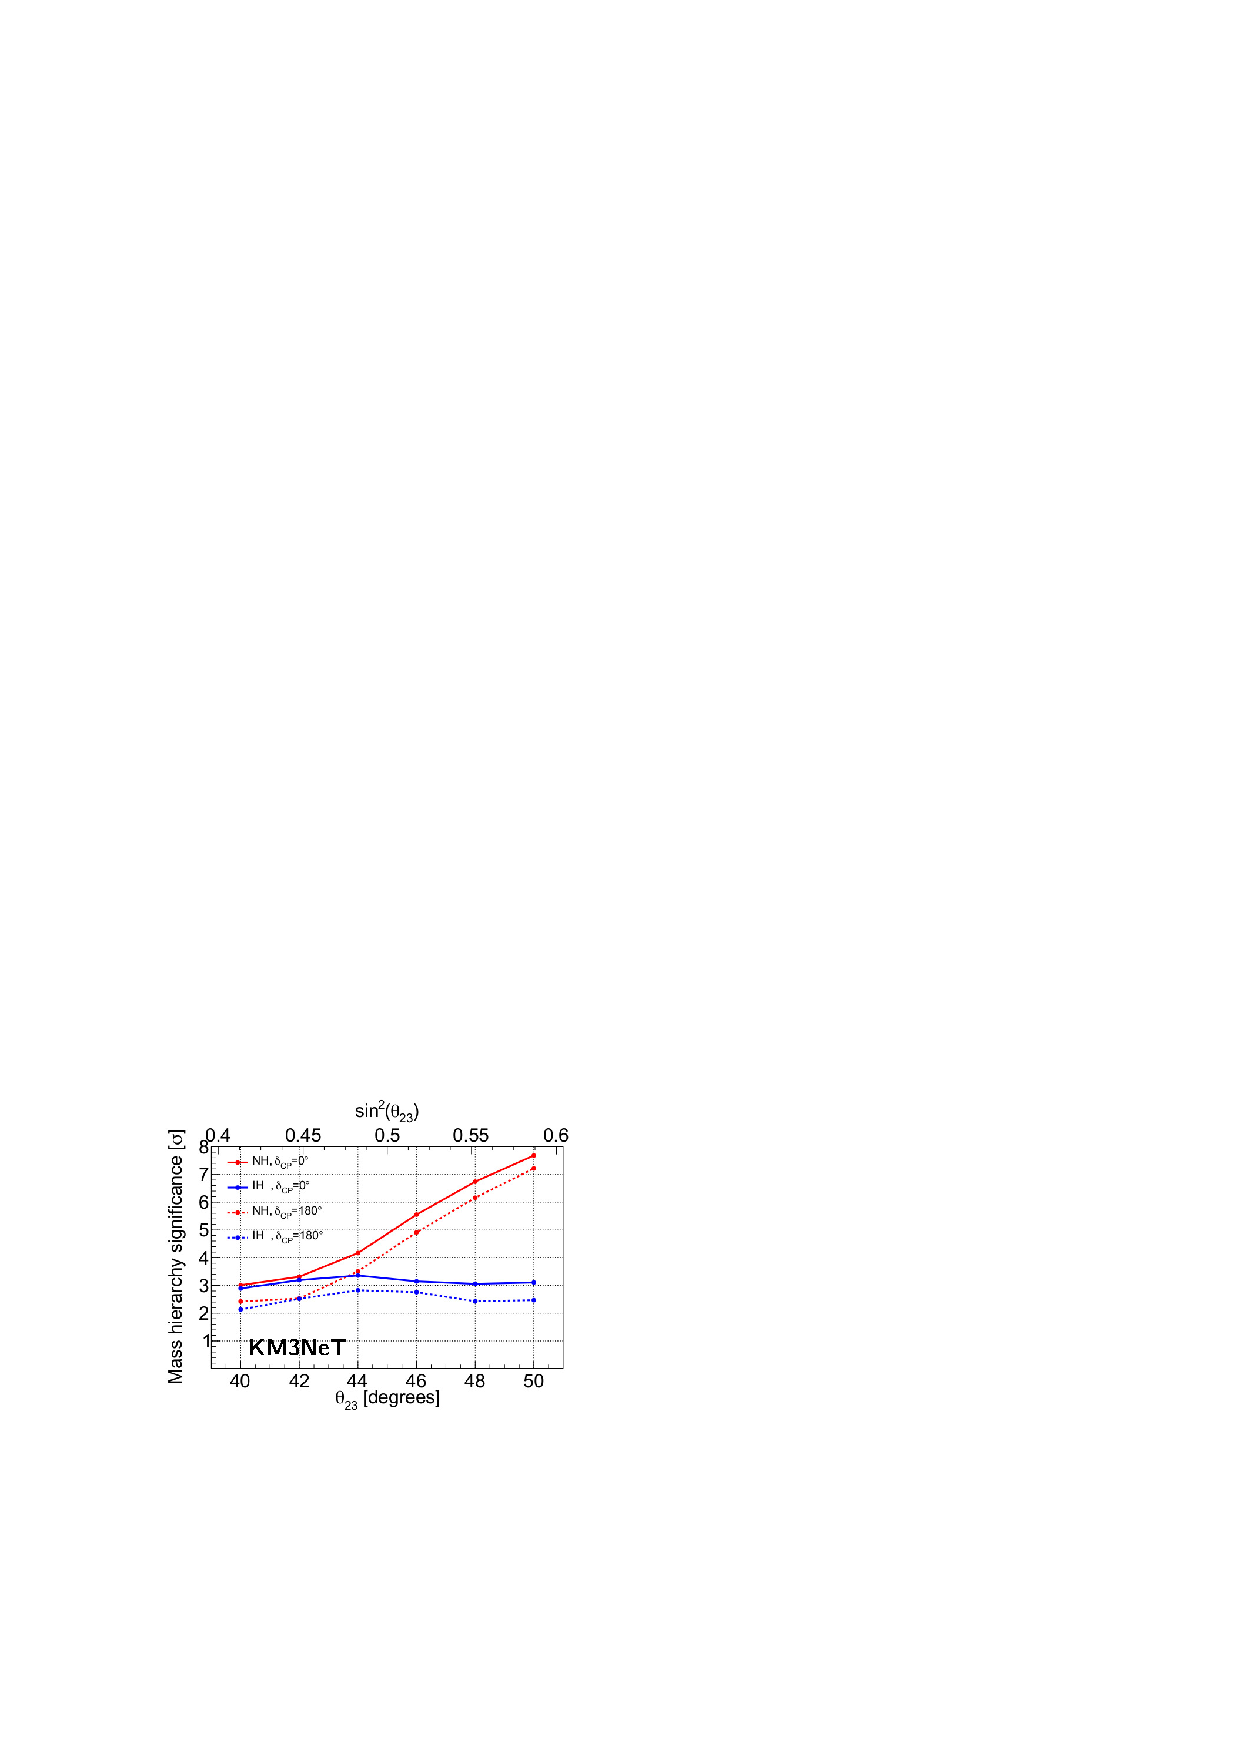
\includegraphics[width=8cm]{figures/orca_sensi.pdf}
\caption{\label{fig:orcasensi} ORCA sensitivity to the mass ordering after three years of running as a function of the true value of \thatm and for different values of \dcp~{Hofestadt:2017jfu}.}
\end{center}
\end{figure}

\begin{figure} [htbp!]
\begin{center}
%add plot!!!
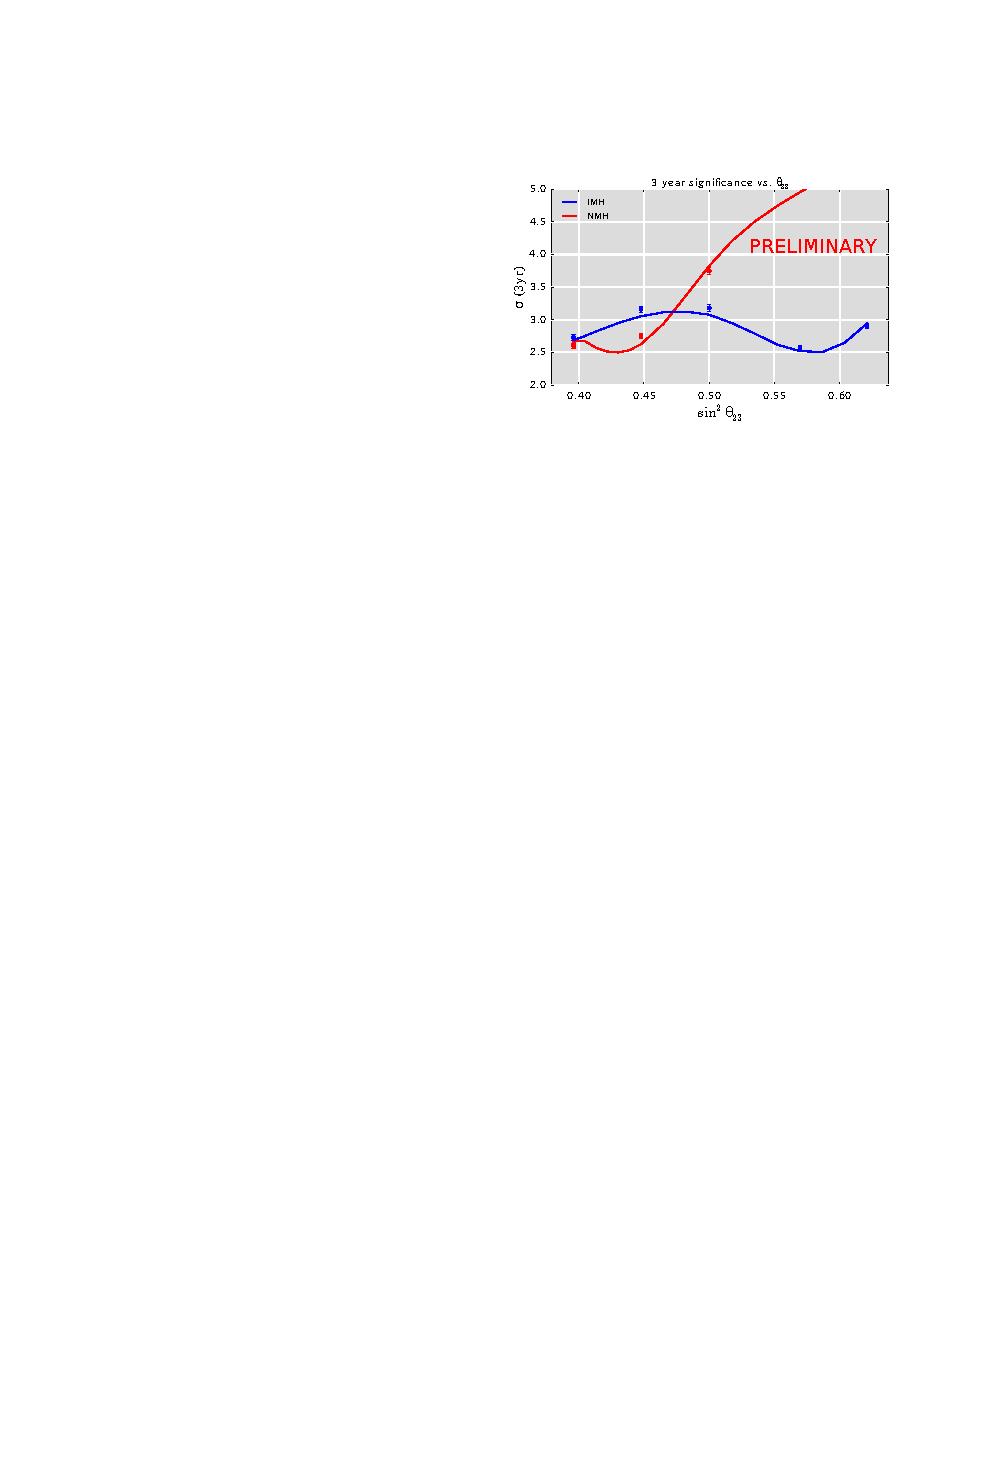
\includegraphics[width=8cm]{figures/pingu_sensi_proceedings.pdf}
\caption{\label{fig:pingusensi} PINGU sensitivity to the mass ordering after three years of running as a function of the true value of \thatm~\cite{Yanez:2016ojt}.}
\end{center}
\end{figure}


Another experiment aimed at determining the mass ordering is the ICAL (Iron Calorimeter)~\cite{Ahmed:2015jtv} detector to be built at the India-based Neutrino Observatory (INO). ICAL will be a 50 kton magnetized detector that will be mainly sensitive to 1-10 GeV atmospheric neutrinos: 5.6 cm thick iron layers are interleaved with Resistive Plate Chambers (RPC) used for tracking the charged particles. Thanks to the 1.5 Tesla magnetic field, ICAL will be capable to reconstruct the charge of the muons, hence separating interaction induced by muon neutrinos from the ones induced by muon antineutrinos.
In order to determine the mass ordering \num and \numb will be binned in momentum and angle, exploiting the matter effects in a similar way as it is proposed by ORCA and PINGU. In the case of INO only muon tracks are used and a sensitivity to the mass ordering of 3 sigma after 10 years of data taking can be obtained.


\subsection{Next generation of long baseline experiments}

The next generation of long-baseline experiments will be built in the coming years and will be operational around the second half of the years 2020 with the main goal of providing precise measurements of the neutrino mixing parameters accessible to long-baseline experiments, namely \thatm, \thint, \dmsq, and \dcp. 
The main goal of these projects will be the discovery of CP violation in the leptonic sector. They will be also able to measure the mass ordering if this will not have been determined by the dedicated experiments described earlier. 

The two existing projects for the next generation of long-baseline are the DUNE experiment in the US and the Hyper-Kamiokande experiment in Japan. Hyper-Kamiokande builds up on the experience with the T2K experiment and the Super-Kamiokande detector. It will be composed by two large water Cherenkov detectors, with a total mass 10 times larger than SK, and it will be exposed to the off-axis neutrino beam produced at JPARC. 
DUNE will use a different and innovative technology by using Liquid Argon as target for neutrino interactions, performing a calorimetric measurement of the tracks produced in neutrino interactions. The collaboration plans to build four modules for a total fiducial mass of 40 kiloton. Neutrinos will be produced at Fermilab, by extracting protons from the Main Ring and will be sent to the Sanford Underground Research Facility (SURF) in South Dakota, 1300 km away from Fermilab.

Both experiments will be multi-purpose detectors, searching for example for proton decays, neutrinos produced in supernova explosions or in supernova remnants, measuring solar and atmospheric neutrinos. In the context of this review we will concentrate on the measurements that will be done by these experiments and that are important for a better understanding of the PMNS matrix.

DUNE will build four large (10 kton of fiducial mass) Liquid Argon time projection chambers as target for neutrino interactions. When neutrinos interact with the Argon, charged particles are produced that cross the medium, ionising and exciting Argon nuclei. This produce both ionization and scintillation signals that are detected by a readout system. The careful collection of the ionization signal allows for a three dimensional reconstruction of the charged tracks and so of the neutrino responsible for the interaction. The collection of the ionization is done with a readout system. Two options are contemplated for the readout of the ionization signals: single-phase readout where the ionization is collected using wire planes in the liquid argon volume and dual-phase approach where the ionization signals are amplified and detected in a gaseous argon region above the liquid. The single-phase readout was the technology used for the ICARUS detector~\cite{CANCI20121257} while for the dual-phase readout several small-scale prototypes have been built in the last years~\cite{}. An extended R\&D program is on-going to demonstrate that both technologies are suitable to build a 10 kton module. Two prototypes, one for the single phase (ProtoDUNE-SP) and one for the dual phase (ProtoDUNE-DP or WA105) of roughly 300 tons and scalable to higher masses are being built at CERN and will be exposed to charged particles beam in 2018.  

\begin{figure} [htbp!]
\begin{center}
%add plot!!!
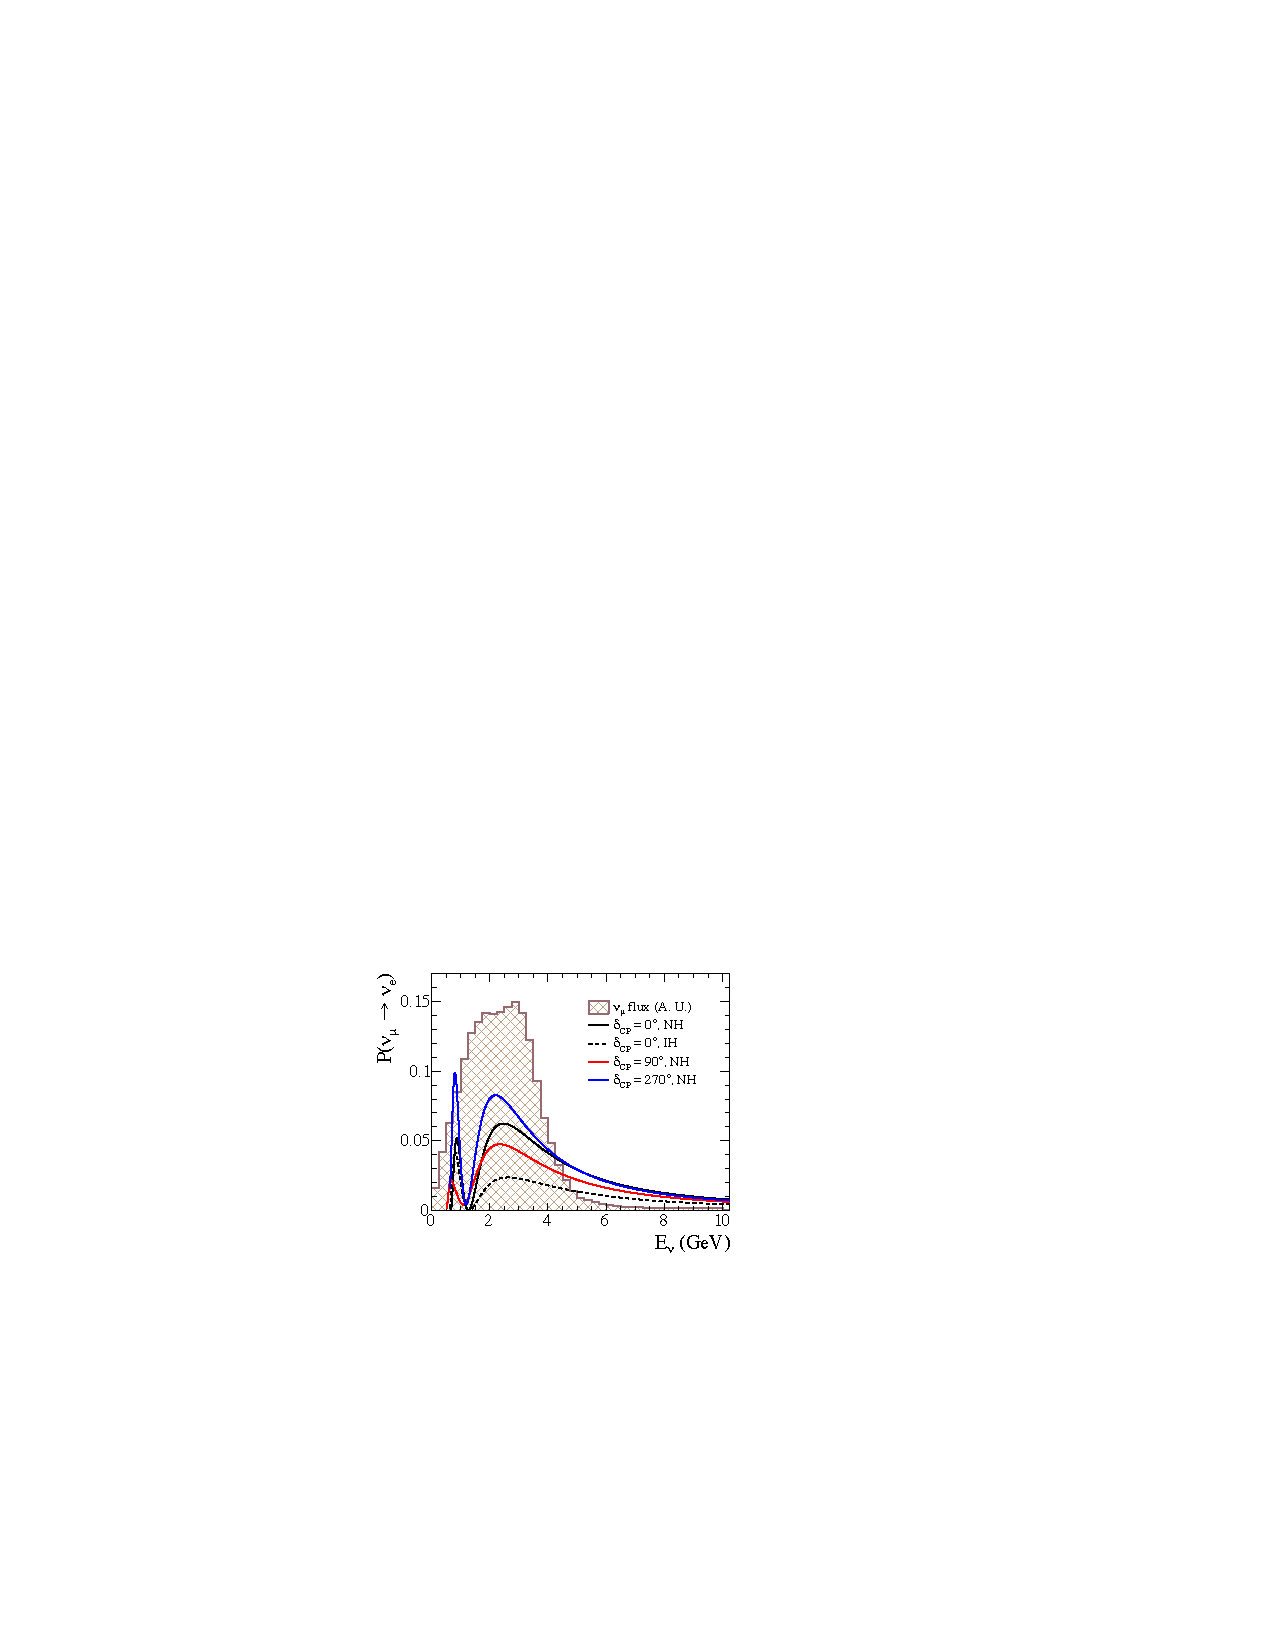
\includegraphics[width=8cm]{figures/dune_flux.pdf}
\caption{\label{fig:duneflux} Oscillation probabilities for different values of mass ordering and \dcp at 1300 km superimposed to the expected DUNE neutrino flux~\cite{Diwan:2016gmz}.}
\end{center}
\end{figure}


The neutrino beam used for DUNE will be a broad band beam produced at the Long Baseline Neutrino Facility (LBNF) at Fermilab. The foreseen beam power is of 1.2~MW. The neutrino flux will cover both the first and the second oscillation maxima, that at 1300 km will be at 2.5~GeV and 0.8~GeV respectively as shown in Fig.~\ref{fig:duneflux}. At energy above 2~GeV, multiple tracks are produced in charged current neutrino interactions and high efficiency to reconstruct all the final state particles is required: the high granularity of a liquid Argon is then better suited at these energies with respect to Water Cherenkov detectors for which most of the charged particles are below the Cherenkov threshold and so cannot be reconstructed.
%In addition the sensitivity to neutrinos at the second maximum is particularly useful because it allows to measure the CP phase from distortions in the energy spectrum.  
Thanks to the very long baseline of DUNE, effects from mass ordering and CP violation are decoupled as shown in Fig.~\ref{fig:novaellipse}. The strategy is to collect neutrino and anti-neutrino data, by changing the sense of the current in the magnetic horns, and measure \num and \numb disappearance and \nue and \nueb appearance probabilities.  
The combination of the four samples allow to have a clean measurement of the mass ordering for any value of \dcp and in both the ordering hypotheses as shown in Fig.~\ref{fig:dunesensi}. As far as the measurement of CP violation is concerned, the sensitivity depends on the value of \dcp. The requirement for the experiment is to have a sensitivity larger than $5~\sigma$ for 50\% of the values of \dcp and larger than $3~\sigma$ for the 75\% of the values of \dcp. Such sensitivities will be reached after XX years of running.

\begin{figure} [htbp!]
\begin{center}
%add plot!!!
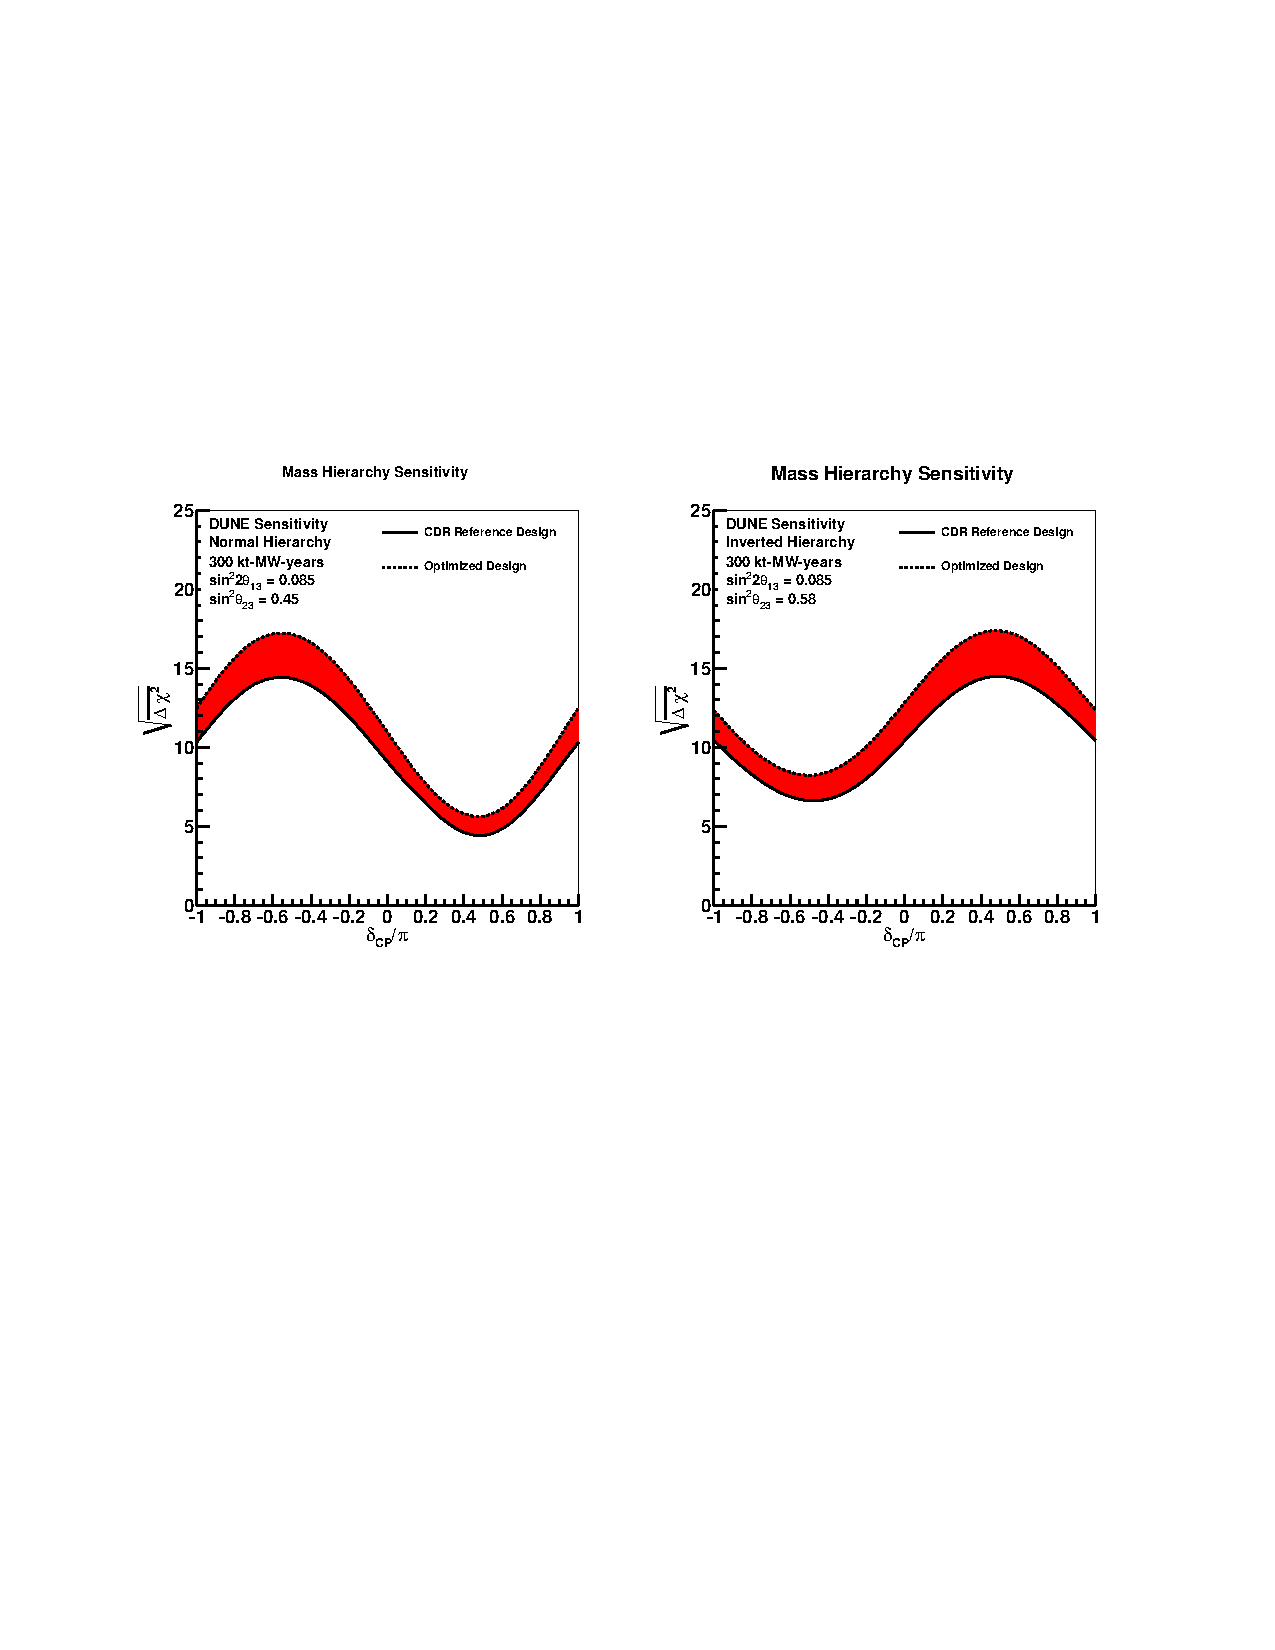
\includegraphics[width=10cm]{figures/dune_MO_sensi.pdf}
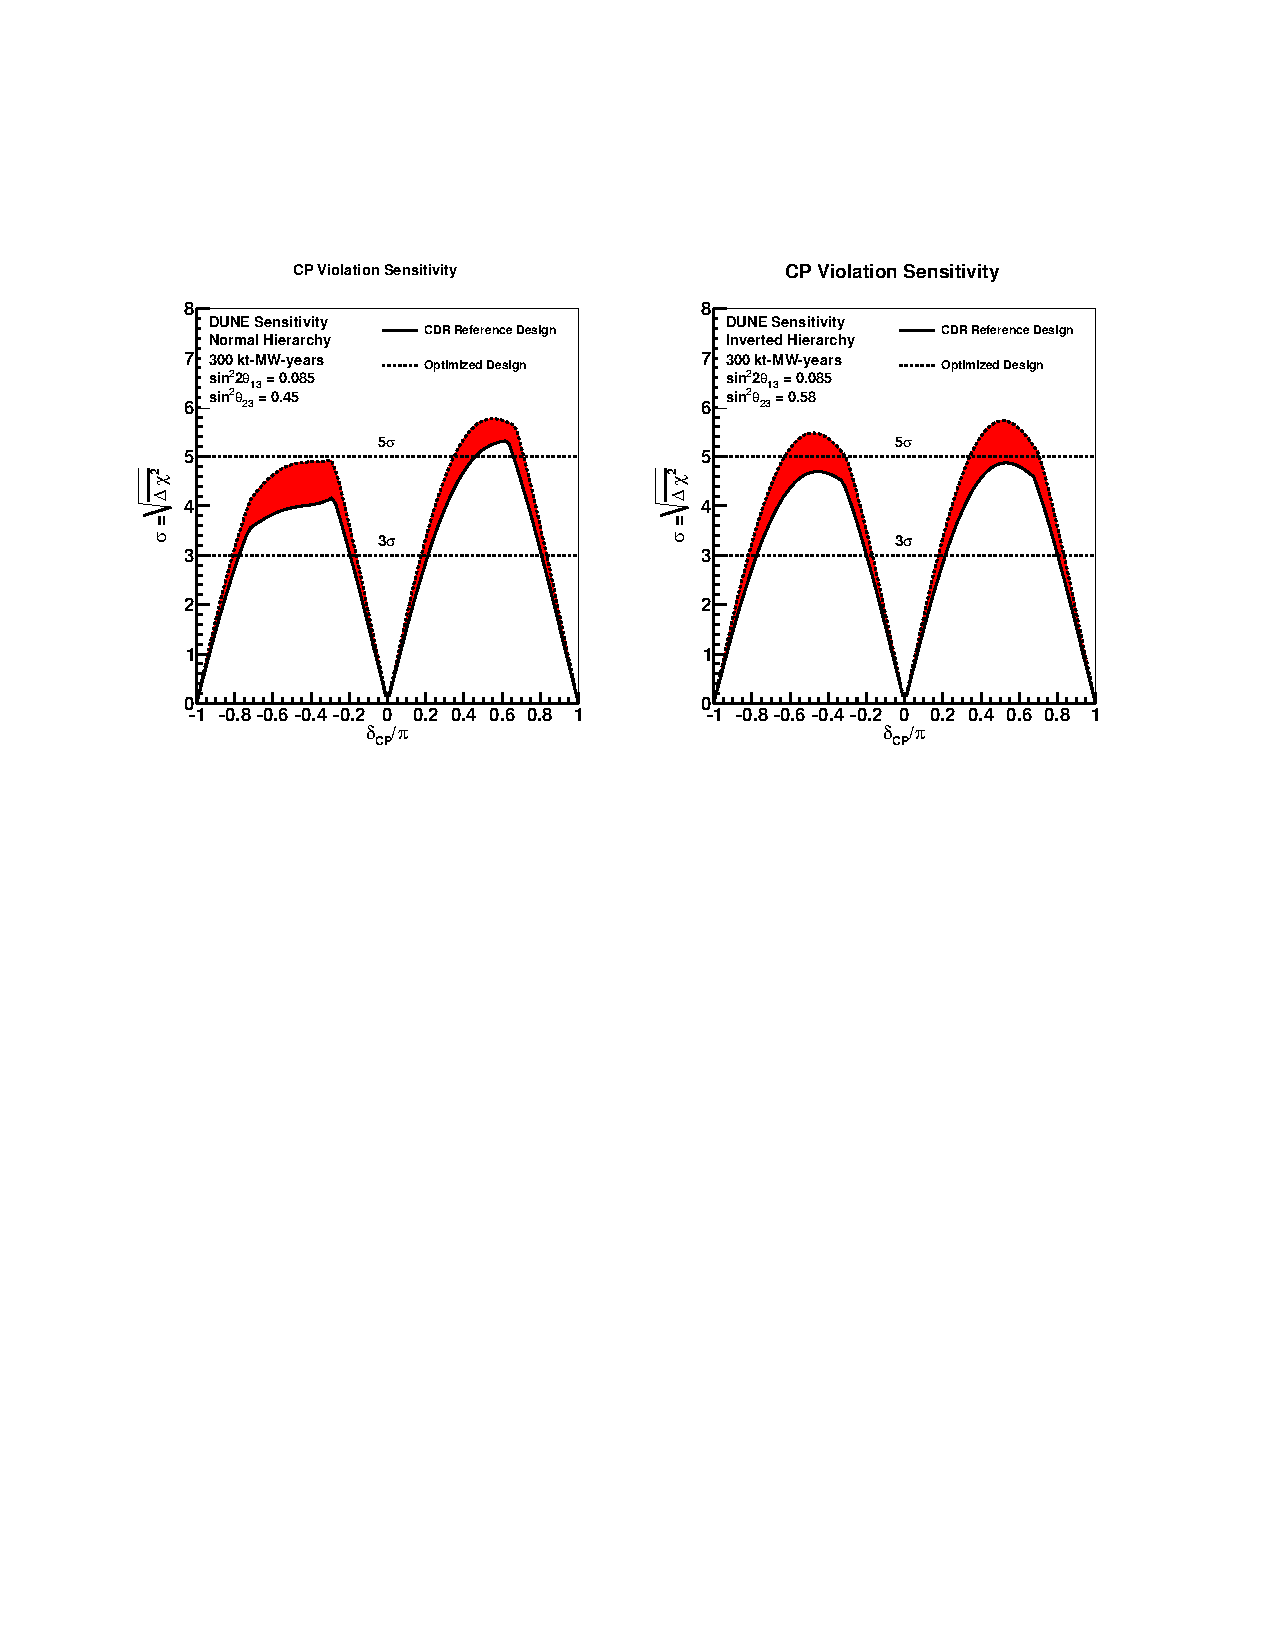
\includegraphics[width=10cm]{figures/dune_CP_sensi.pdf}
\caption{\label{fig:dunesensi} DUNE expected sensitivity to the mass ordering (top) and the CP violation phase (bottom) for normal (left) and inverted (right) ordering for an exposure of 300~kt$\times$MW$\times$year~\cite{Acciarri:2015uup}.}
\end{center}
\end{figure}


The other proposed long-baseline experiment is Hyper-Kamiokande (HK). The current design of HK is to have a staged construction of two 187~kton fiducial volume mass modules near the current Super-Kamiokande site at a distance of 295~km and 2.5 degrees off-axis from the J-PARC site where neutrinos are produced. The neutrino beam is the same currently used by the T2K experiment but, thanks to an upgrade of the JPARC Main Ring power supplies, it will be able to operate at more than 1.3~MW  by 2025 (the beam power today is 470~kW).

The baseline design  for Hyper-Kamiokande is to have the two modules at Kamioka but an alternative design is being pursued to install the second module in South Korea~\cite{Abe:2016ero}. This second detector would be operated at a baseline of roughly 1100~km and a smaller off-axis angle. In this configuration HK would be sensitive to the first and the second oscillation maxima, with the first taking place at $\sim2~GeV$ and the second at $0.6~GeV$. In this configuration the first oscillation maximum would give sensitivity to the mass ordering while the second would allow to exploit the larger CP asymmetry, improving the measurement of \dcp.  If both detectors will be installed at Kamioka, external measurements of the mass ordering will be used in the search for \dcp. If no measurements of mass ordering will be available by the time HK is collecting data, the mass ordering can still be determined at more than $3~\sigma$ by measuring matter effects in the large atmospheric neutrino sample that will be collected in HK.    

After 10 years of data taking  HK will collect $\sim1000$ ($\sim130$) \nue and \nueb signal events per tank at 295 km (1100 km and 2.0 degrees off-axis) assuming a 3:1 ratio of antineutrino mode to neutrino mode operation. The sensitivity of the experiment for different options for the location of the second tank is shown in Fig.~\ref{fig:hkcpv}. From the figure it is clear the benefit of the second detector in Korea if no measurements of the mass ordering will be available by 2025. On average, the second detector in Korea, also allows for a more precise measurement of the value of \dcp, thanks to the exploitation of the second maximum. A precision between 6 and 13 degrees can be obtained depending on the value of \dcp. Finally the sensitivity in Korea will be limited by statistical uncertainties even after 10 years of data taking while in Kamioka the measurements will be limited by systematic uncertainties.

\begin{figure} [htbp!]
\begin{center}
%add plot!!!
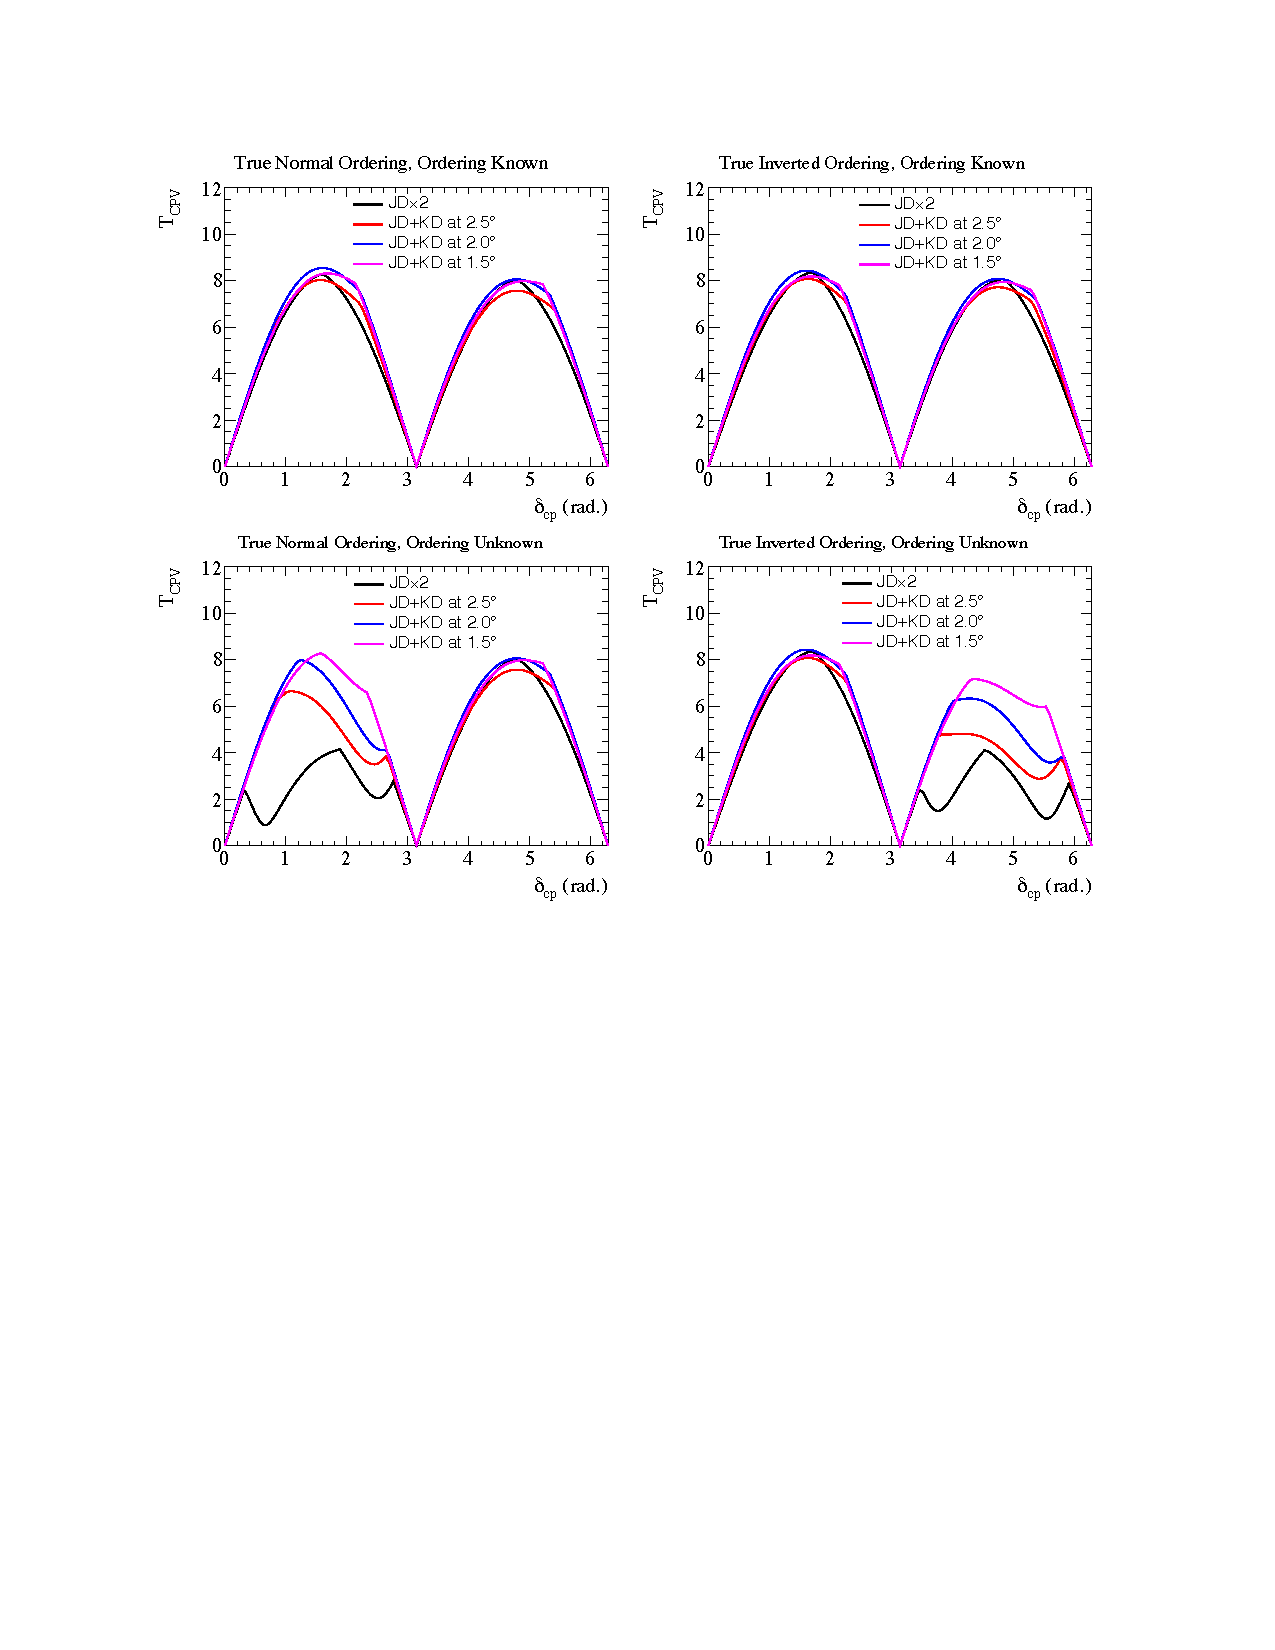
\includegraphics[width=15cm]{figures/hk_cpv_sensi.pdf}
\caption{\label{fig:hkcpv} Significance to reject CP conservation as a function of \dcp for normal ordering (left) and inverted ordering (right) and different hypotheses for the location of the second tank. On the top row the mass ordering is assumed to be known independentely from accelerator based neutrinos, on the bottom row the mass ordering is unknown~\cite{Abe:2016ero}.}
\end{center}
\end{figure}


HyperK 500 kt fiducial (finance ?) upgraded T2K beam

complementarity DUNE/HK